%%%%%%%%%%%%%%%%%%%%%%%%%%%%%%%%%%%%%%%%%
% Masters/Doctoral Thesis 
% LaTeX Template
% Version 1.42 (19/1/14)
%
% This template has been downloaded from:
% http://www.latextemplates.com
%
% Original authors:
% Steven Gunn 
% http://users.ecs.soton.ac.uk/srg/softwaretools/document/templates/
% and
% Sunil Patel
% http://www.sunilpatel.co.uk/thesis-template/
%
% License:
% CC BY-NC-SA 3.0 (http://creativecommons.org/licenses/by-nc-sa/3.0/)
%
% Note:
% Make sure to edit document variables in the Thesis.cls file
%
%%%%%%%%%%%%%%%%%%%%%%%%%%%%%%%%%%%%%%%%%

%----------------------------------------------------------------------------------------
%	PACKAGES AND OTHER DOCUMENT CONFIGURATIONS
%----------------------------------------------------------------------------------------

\documentclass[11pt, a4paper, oneside]{Thesis} % Paper size, default font size and one-sided paper

\graphicspath{{Pictures/}} % Specifies the directory where pictures are stored

\usepackage[square, numbers, comma, sort&compress]{natbib} % Use the natbib reference package - read up on this to edit the reference style; if you want text (e.g. Smith et al., 2012) for the in-text references (instead of numbers), remove 'numbers' 
\usepackage{rotating}
\usepackage{fontspec}
\setmainfont{Open Sans}
\usepackage{longtable}


\hypersetup{urlcolor=black,citecolor=black, linkcolor=black, colorlinks=true} % Colors hyperlinks in blue - change to black if annoying
\title{\ttitle} % Defines the thesis title - don't touch this

\begin{document}

\frontmatter % Use roman page numbering style (i, ii, iii, iv...) for the pre-content pages

\setstretch{1.5} % Line spacing of 1.5

% Define the page headers using the FancyHdr package and set up for one-sided printing
\fancyhead{} % Clears all page headers and footers
\rhead{\thepage} % Sets the right side header to show the page number
\lhead{} % Clears the left side page header

\pagestyle{fancy} % Finally, use the "fancy" page style to implement the FancyHdr headers

\newcommand{\HRule}{\rule{\linewidth}{0.5mm}} % New command to make the lines in the title page

% PDF meta-data
\hypersetup{pdftitle={\ttitle}}
\hypersetup{pdfsubject=\subjectname}
\hypersetup{pdfauthor=\authornames}
\hypersetup{pdfkeywords=\keywordnames}

%----------------------------------------------------------------------------------------
%	TITLE PAGE
%----------------------------------------------------------------------------------------

\begin{titlepage}

\begin{center}

\textsc{\LARGE \univname}\\[1.5cm] % University name
\textsc{\Large Masters Dissertation}\\[0.5cm] % Thesis type

\HRule \\[0.4cm] % Horizontal line
{\huge \bfseries \ttitle}\\[0.4cm] % Thesis title
\HRule \\[1.5cm] % Horizontal line
 
\begin{minipage}{0.4\textwidth}
\begin{flushleft} \large
\emph{Author:}\\
\authornames % Author name - remove the \href bracket to remove the link
\end{flushleft}
\end{minipage}
\begin{minipage}{0.4\textwidth}
\begin{flushright} \large
\emph{Supervisor:} \\
\supname % Supervisor name - remove the \href bracket to remove the link  
\end{flushright}
\end{minipage}\\[2cm]

\large \textit{Dissertation submitted in partial fulfilment of the requirements\\ for the degree of \degreename}\\[0.3cm] % University requirement text
\textit{in the}\\[0.4cm]
\deptname\\[2cm] % Research group name and department name
{\large \today}\\[2cm] % Date
 \begin{figure}[h!]
 \centering
 \includegraphics[width=4cm]{Figures/uctlogo.jpg} 
 \hspace{2cm} 
 \includegraphics[width=3cm]{Figures/compsci.jpg}  
 \end{figure} 

\end{center}

\end{titlepage}

%----------------------------------------------------------------------------------------
%	DECLARATION PAGE
%	Your institution may give you a different text to place here
%----------------------------------------------------------------------------------------

\Declaration{

\addtocontents{toc}{\vspace{1em}} % Add a gap in the Contents, for aesthetics

I, \authornames, declare that this dissertation titled, '\ttitle' and the work presented in it are my own. I confirm that:

\begin{itemize} 
\item[\tiny{$\blacksquare$}] This work was done wholly while in candidature for a research degree at this University.
\item[\tiny{$\blacksquare$}] Where I have consulted the published work of others, this is always clearly attributed.
\item[\tiny{$\blacksquare$}] Where I have quoted from the work of others, the source is always given. With the exception of such quotations, this dissertation is entirely my own work.
\item[\tiny{$\blacksquare$}] I have acknowledged all main sources of help.

\item[\tiny{$\blacksquare$}] I know the meaning of plagiarism and declare that all of the work in this dissertation, save for that which is properly acknowledged, is my own.\\
\end{itemize}
 
Signed:\\
\rule[1em]{25em}{0.5pt} % This prints a line for the signature
 
Date:\\
\rule[1em]{25em}{0.5pt} % This prints a line to write the date
}




\clearpage % Start a new page

%----------------------------------------------------------------------------------------
%	COPYRIGHT
%----------------------------------------------------------------------------------------


\licensing{\addtocontents{toc}{\vspace{1em}}
 \authornames~ is the author of this dissertation, and holds copyright in terms of the University of Cape Town's Intellectual Property Policy, July 2011.\\ (\href{http://www.uct.ac.za/downloads/uct.ac.za/about/policies/intellect_property.pdf}{http://www.uct.ac.za/downloads/uct.ac.za/about/policies/intellect\_property.pdf}).\\
\\
 This work is licensed by the author under a Creative Commons Attribution 2.5 South Africa License. (\href{http://creativecommons.org/licenses/by/2.5/za/deed.en}{http://creativecommons.org/licenses/by/2.5/za/deed.en}).
 \begin{center}
   \includegraphics[width=3cm]{Figures/cc-by.jpg}	
 \end{center}


 \clearpage
 

}



%----------------------------------------------------------------------------------------
%	QUOTATION PAGE
%----------------------------------------------------------------------------------------

\pagestyle{empty} % No headers or footers for the following pages

\null\vfill % Add some space to move the quote down the page a bit


\textit{"All of Computer Science is a subset of Human-Computer Interaction."}

\begin{flushright}
Gary Marsden
\end{flushright}

\vfill\vfill\vfill\vfill\vfill\vfill\null % Add some space at the bottom to position the quote just right

\clearpage % Start a new page

%------------------2----------------------------------------------------------------------
%	ABSTRACT PAGE
%----------------------------------------------------------------------------------------

\addtotoc{Abstract} % Add the "Abstract" page entry to the Contents
\vspace{-5em}
\abstract{\addtocontents{toc}{\vspace{1em}} % Add a gap in the Contents, for aesthetics

Systems to annotate online content are becoming increasingly common on the World Wide Web. While much research and development has been done for interfaces that allow users to make and view annotations, few annotation systems provide functionality that extends beyond this and allows users to also manage and process collections of existing annotations.\\
\\
Siyavula Education is a social enterprise that publishes high school Maths and Science textbooks online. The company uses annotations to collate collaborator and volunteer feedback (corrections, opinions, suggestions) about its books at various phases in the book-writing life cycle.  \\
\\
Currently the company captures annotations on PDF versions of their books. The web-based software they use allows for some filtering and sorting of existing annotations, but the system is limited and not ideal for their rather specialised requirements. \\
\\
In an attempt to move away from a proprietary, PDF-based system Siyavula implemented Annotator (\href{http://okfnlabs.org/annotator/}{http://okfnlabs.org/annotator/}), software which allowed for the annotation of HTML pages. However, this software was not coupled with a back-end interface that would allow users to interact with a database of saved annotations. \\
\\
To enable this kind of interaction, a prototype interface was designed and is presented here. The purpose of the interface was to give users new and improved functionality for querying and manipulating a collection of web-based annotations about Siyavula’s online content.\\
\\
Usability tests demonstrated that the interface was successful at giving users this new and necessary functionality (including filtering, sorting and searching) to process annotations. \\ 
\\
Once integrated with front-end software (such as Annotator) and issue tracking software (such as GitHub) the interface could form part of a powerful new tool for the making and management of annotations on the Web. 
}

\clearpage % Start a new page

%----------------------------------------------------------------------------------------
%	ACKNOWLEDGEMENTS
%----------------------------------------------------------------------------------------

\setstretch{1.3} % Reset the line-spacing to 1.3 for body text (if it has changed)

\acknowledgements{\addtocontents{toc}{\vspace{1em}} % Add a gap in the Contents, for aesthetics

The completion of this dissertation (and the rest of my degree) would not have been possible without the endless love, support and encouragement of my partner Ewald, my parents Jill and Pierre and my extended family and friends who are too numerous to name individually. To Ewald particularly, multiverses of gratitude and love are due not only for help with the back-end development involved in this research, but also for putting up with much grumpiness, impatience and exhaustion. I could not have completed this thesis without his support and sanity-restoring advice. \\
\\
Thanks are also due to my employers, colleagues and friends at Siyavula for giving me the time and space to do this research and being extremely willing and enthusiastic users.\\
\\
My extraordinary supervisor, Gary Marsden, passed away suddenly just weeks before I was due to submit this dissertation. The loss of Gary is a profound tragedy for his family, his students, his colleagues and the HCI community at large. While I grieve for him still and there will forever be a Gary-shaped hole in the universe (to paraphrase Arundhati Roy) I am honoured to have been one of his "minions" and will always be grateful for the time I had with him. I only wish he could see this work in its completed form. 

I am indebted to Associate Professor Sonia Berman (UCT) and Professor Yvonne Rogers (University College London), who helped me through the last few weeks of this process and gave me invaluable advice and encouragement. 

On a lighter note, acknowledgement for completion of this dissertation must also be given to Daft Punk and Swedish House Mafia: because sometimes one just needs a heavy beat to get things done.

}


\clearpage % Start a new page

%----------------------------------------------------------------------------------------
%	LIST OF CONTENTS/FIGURES/TABLES PAGES
%----------------------------------------------------------------------------------------

\pagestyle{fancy} % The page style headers have been "empty" all this time, now use the "fancy" headers as defined before to bring them back

\lhead{\emph{Contents}} % Set the left side page header to "Contents"
\tableofcontents % Write out the Table of Contents

\lhead{\emph{List of Figures}} % Set the left side page header to "List of Figures"
\listoffigures % Write out the List of Figures

\lhead{\emph{List of Tables}} % Set the left side page header to "List of Tables"
\listoftables % Write out the List of Tables

%----------------------------------------------------------------------------------------
%	ABBREVIATIONS
%----------------------------------------------------------------------------------------

% \clearpage % Start a new page
% 
% \setstretch{1.5} % Set the line spacing to 1.5, this makes the following tables easier to read
% 
% \lhead{\emph{Abbreviations}} % Set the left side page header to "Abbreviations"
% \listofsymbols{ll} % Include a list of Abbreviations (a table of two columns)
% {
% \textbf{LAH} & \textbf{L}ist \textbf{A}bbreviations \textbf{H}ere \\
% %\textbf{Acronym} & \textbf{W}hat (it) \textbf{S}tands \textbf{F}or \\
% }



%----------------------------------------------------------------------------------------
%	DEDICATION
%----------------------------------------------------------------------------------------

\setstretch{1.3} % Return the line spacing back to 1.3

\pagestyle{empty} % Page style needs to be empty for this page

\dedicatory{This dissertation is dedicated to the memory of Gary Marsden: the finest supervisor and mentor a student could hope to have.} % Dedication text

\addtocontents{toc}{\vspace{2em}} % Add a gap in the Contents, for aesthetics

%----------------------------------------------------------------------------------------
%	THESIS CONTENT - CHAPTERS
%----------------------------------------------------------------------------------------

\mainmatter % Begin numeric (1,2,3...) page numbering

\pagestyle{fancy} % Return the page headers back to the "fancy" style

% Include the chapters of the thesis as separate files from the Chapters folder
% Uncomment the lines as you write the chapters

\part{Introduction}
% Chapter 1

\chapter{Introduction} % Main chapter title

\label{Chapter1} % For referencing the chapter elsewhere, use \ref{Chapter1} 

\lhead{Chapter 1. \emph{Introduction}} % This is for the header on each page - perhaps a shortened title

%----------------------------------------------------------------------------------------

\section{Introduction}
Siyavula Education is a Cape Town-based social enterprise that publishes open source high school maths and science textbooks. The books are written collaboratively by volunteers and then edited and refined in-house. The volunteer community plays a central role in the book making process. Volunteers contribute towards authoring new content, editing existing content, proofreading and translation. The final versions of the books are available as printed hard copies, PDF downloads and as webbooks, which can be read online using a variety of devices. 

One mechanism by which volunteers, or any member of the public, can give Siyavula feedback is via annotations. This is not only a tool for flagging small errata in the books; Siyavula also uses annotations to get feedback from volunteers during the authoring process, and during the editing and proofreading phases.


\subsection{Current annotation system}

Currently, Siyavula uses the web-based software a.nnotate.com\footnote{\href{ http://a.nnotate.com/}{ http://a.nnotate.com/}}. To use this system the company must upload draft PDFs of a particular chapter of a book, and external users (who have been given the necessary permissions) can then view, highlight and make comments on the content. Users can select a particular "type" for their comment (error, comment or suggestion) and they can also add custom tags to comments. Any user who has access to a particular PDF can view and reply to all annotations made on the document. 

A.nnotate.com is not very easy to use for volunteers who need to make annotations: pages are often slow to load (especially for large documents, and a single chapter of a book may be anywhere between 20 and 90 pages long) and the interface is not intuitive, particularly for less advanced computer users. Similarly, it is not user-friendly for the Siyavula team members who have to process or capture annotations that have been made. 

'Processing' an annotation involves an employee locating an annotation in the context of a book (or subject or grade), assessing its validity (e.g. "\textit{is there really an error in the text as flagged by a volunteer?}''), making changes to the book content's source code if necessary and somehow marking that annotation as resolved.

To do this currently, employees have to trawl through the uploaded PDF documents one page at a time to view annotations in the context in which they were made. Whilst a.nnotate.com offers basic filtering, searching and sorting of notes, this functionality is predetermined (and limited) and not customised to Siyavula's workflow. For example, there is no efficient way to mark annotations as resolved or to lock down a particular annotation and its replies (one can only prevent access to the entire document). It is not possible to view annotations with a preview of the the text to which they relate and it is not possible to group annotations by subject (e.g. Maths), type or username, or to cross-reference annotations between different PDFs. There have also been problems with old annotations simply being deleted from the a.nnotate.com database.  


\subsection{New annotation system}

Due to the limited functionality of a.nnotate.com (software arguably not designed for the kind of functionality that Siyavula requires from it); its proprietary nature (one has to pay to upload documents over a certain file size); and the fact that it can only handle PDF documents, it was decided that Siyavula would implement its own annotation software on the company's websites. This would allow Siyavula to develop the software according to its own rather specialised needs and to capture annotations on (HTML) web versions of the books, not merely PDFs.  

For external users, the beta version of Siyavula's new annotator behaved in much the same way as a.nnotate.com, albeit with a simpler, cleaner interface. The software allowed users to highlight text in a static webpage and make an annotation about that text, in one of three categories: "errata'', "comment'' and "suggestion''. 

These annotations were then stored in a database, and could be viewed by employees in a table  with the most recent annotations listed first. 
%---------------------------------------------------------------------------------------------------------------------

\section{The problem}
The very limited back-end interface (a single table) provided by the new annotation software did not include any functionality for Siyavula team members to filter, search, sort or process annotations that have been made. Users could scroll through the contents of the table, but had no tools whatsoever to manipulate or interact with the information provided. Users had no way of meaningfully and efficiently engaging with the existing system and stored annotation content.



%----------------------------------------------------------------------------------------

\section{The solution}
The solution to the above problem was to develop a new interface customised to Siyavula's requirements that would provide team members with new functionality to engage with existing annotations. 

Being able to filter, search for, and sort existing annotations would enable users to locate sets or subsets of annotations, to find individual annotations, or to view particular details about a single annotation or user, all previously impossible tasks. Such functionality could streamline the ways in which team members process and resolve annotations made by volunteers and external users.

A user-centred approach was adopted to identify and answer specific questions about user requirements and to include user feedback in as many stages of the design process as possible. Once the high-fidelity prototype was complete, user-centred evaluation was also undertaken in order to determine whether or not the final prototype properly met user requirements and expectations and adequately provided them with new and desired functionality for processing annotations. 

\section{Scope of the research}
The scope of this research was limited to solving Siyavula's problem specifically. The interface was designed to meet the requirements of a niche group of users, and to fit into their unique existing annotation-processing pipeline and software system. However, the final interface exists independently of any underlying software and could therefore easily be assimilated into a different system or process. This software independence is desirable for Siyavula because it allows room for their underlying annotation software and database to change. It also means that the interface could be repurposed for other organisations' requirements.

At the time of writing, Siyavula's use of annotations to capture volunteer feedback on web-based textbooks appears to be unique in the realm of open education and publishing. Nonetheless, in future this kind of workflow may well be adopted by similar organisations or those using annotations as tools in a structured process. If so, the need for an interface to enable users to engage with such content may become more widespread. 

%----------------------------------------------------------------------------------------

\section{The structure of this dissertation}

Chapter 2 provides more technical details about Siyavula's annotation software and its functionality. Chapter 3 provides an overview of existing research in this field. Chapter 4 outlines the user-centred methodology, tools and design guidelines used in the development of the interface. Chapter 5 deals with the design process while Chapter 6 covers the technical details about development of the high-fidelity prototype. Chapter 7 deals in detail with the process of user-centred evaluation and iterative improvements to and testing of the interface. The success of the final interface and future work are discussed in Chapter 8.   

% Chapter 2

\chapter{The Existing Annotator System} % Main chapter title

\label{Chapter2} % For referencing the chapter elsewhere, use \ref{Chapter1} 

\lhead{Chapter 2. \emph{The Existing Annotator System}} % This is for the header on each page - perhaps a shortened title

%----------------------------------------------------------------------------------------

\section{Overview of Annotator}
The beta version of Siyavula's Annotator software allowed people to highlight HTML text in a webbook and make an annotated comment about their selection. In order to use the annotator, users had to be be logged in so that their annotations could be correctly attributed to them. 

\begin{figure}[h]
    \centering
    \includegraphics[width=0.4\textwidth]{Figures/annotator1.png}
 \caption{Highlighted text with the "Annotate'' icon}
\end{figure}

Annotations could be made in one of three categories: errata, suggestion and comment.
\begin{figure}[h]
    \centering
    \includegraphics[width=\textwidth]{Figures/annotatorcategories.png}
 \caption{Three categories of annotation}
\end{figure}

They were then stored in a database for future reference. All users could view existing annotations on a webpage when they logged into the annotated version of the webbook. Users could also reply to existing annotations made by themselves or other users.

%-----------------------------------------
\section{Technical details of Annotator}
The annotation software Siyavula decided to utilise (and modify for the company's own purposes) is based on an open source application called "Annotator"\footnote{\href{ http://okfnlabs.org/annotator/}{ http://okfnlabs.org/annotator/}} (forked by Siyavula's developer at \href{https://github.com/ezietsman/annotator}{https://github.com/ezietsman/annotator}). Annotator is a Javascript application that is written in CoffeeScript\footnote{\href{http://coffeescript.org/}{http://coffeescript.org/}}. It uses CouchDB\footnote{\href{http://couchdb.apache.org/}{http://couchdb.apache.org/}} and has a Python server back-end. It does not come packaged with any functional user interface for the viewing of saved annotations outside of the webpage where they were made.

Siyavula's version of Annotator ran on static versions of the company's webbooks, not on the latest live versions.

%-----------------------------------------
\section{Existing interface}
The back-end interface for the annotator consisted of a simple table list of annotations.

Table columns included: "Type", "id" (the database primary key), "Comment" (the text typed by the user), "User", "Time" (date and time) and "URL" (the webpage on which the annotation was made.) Most recent annotations were listed first. The type of annotation was also indicated by one of three colours in the left-hand column.
\begin{figure}[h]
    \centering
    \includegraphics[width=\textwidth]{Figures/annotator-backend-table.png}
 \caption{The existing back-end interface: a simple table of stored annotation data}
\end{figure}

Columns were not sortable, and there was no search or filter mechanism. The back-end merely provided a list of annotations, with some basic information about each entry. For in-house processing of small numbers of annotations ( $<$ 20), this basic back-end was adequate (albeit  very rough) for advanced members of the team. However, this interface was not scalable (processing $>$ 100 annotations listed like this would be extremely difficult) and not user-friendly at all, particularly for less technologically advanced employees. Indeed, it had not been designed with any user requirements in mind at all - it had merely been cobbled together as a temporary way to view annotations that had been made.

Given the simplicity of the existing interface and the potential for a functional annotator to be an integral part of many stages of Siyavula's book-writing and -maintaining process, it was decided that there would be immense value in designing a unique back-end interface. This interface could be tailored to accommodate different team members' specific user requirements and therefore help to maximise the use of the annotator as a functional tool for making, storing, processing and resolving annotations containing volunteer and general feedback.
 
% Chapter 3

\chapter{Related Research} % Main chapter title

\label{Chapter3} % For referencing the chapter elsewhere, use \ref{Chapter1} 

\lhead{Chapter 3. \emph{Related Research}} % This is for the header on each page - perhaps a shortened title

%----------------------------------------------------------------------------------------

%add a synthesis or “see the wood for the trees” thread that runs through it, or both.  chapter 3 might need some re-writing to slant it more towards “Related Research” rather than What Tools Exist. 

%Edit a bit with a higher-level thread. 

%maybe you could also include other research on how users use search and filter tools for finding and sorting content from databases. As what you are planning to do is not provide more or different annotation tools but the capability to sort and categorize them.

%find 2 or 3 summary papers - one papra on research re finding and sorting content from DBs

The Concise Oxford English Dictionary describes an annotation as an explanatory note added to a book or document \citep{OxfordDict}. Haslhofer et al \citep{LEMO} extend this and state that an annotation can be seen as ``a remark, explanation or interpretation added to the original document". According to Ovsiannikov et al \citep{Ovsiannikov} annotations may take the form of written notes, a symbol, a drawing or, in the digital space, a multimedia clip. 

Analogue annotations and marginalia in books and other hardcopy documents have a long tradition \citep{LEMO} and come in a variety of formats (some more formal than others) including handwritten notes in margins, printed margin notes in textbooks and Post-it notes stuck on to content. More recently, with the inevitable shift towards digital reading, annotations have become possible in desktop software suites, on e-reading devices such as Amazon's Kindle, and on the World Wide Web. 

Much research has been done into the different types of annotations that exist \citep{Marshall2000} \citep{Marshall2004}, the workflows by which they are created, and their purpose and usage  particularly in the digital realm \citep{Agosti} \citep{Ovsiannikov}. Agosti et al. \citep{Agosti} name three major uses for annotations: to create new information resources, to interpret existing ones, to access resources in new ways, and to support the effective use of resources.  Arko et al. \citep{Arko} state that annotations also allow for community engagement and the capturing of ``ephemeral information" that would otherwise be ``lost in transient media like conversation" or emails. This is applicable to analogue annotations, but is particularly true of digital annotations, which can so easily be shared, viewed and processed online.

While desktop software to make and read annotations (or ``notes" or ``comments") has been around for years (e.g. MSOffice \citep{MSOffice} for Microsoft documents, and Adobe Reader \citep{Adobe} for PDFs), a multitude of new technologies are becoming available due to increasing interconnectivity and new storage options given to us by the Web. Examples of online annotation software include Google Drive \citep{GDrive} (for documents and spreadsheets), A.nnotate.com \citep{AnnotateCom} and AnnotateIt \citep{AnnotateIt}.

As online annotation possibilities have expanded, a number of frameworks have been developed to try and standardise the ways in which annotations can me made, stored and manipulated, particularly on the Semantic Web \citep{Berners-Lee} \citep{Uren}. Notable examples of such frameworks include Annotea \citep{kahan2002annotea}, CREAM \citep{handschuh2002authoring} and LEMO \citep{LEMO}.  

A number of online annotation systems have emerged out of these frameworks. The vast majority are concerned with creating and viewing annotations. Only a handful go beyond this and deal with annotation management. Many of these front-end systems have been analysed and compared extensively by Kahan et al \citep{kahan2002annotea} and Haslhofer et al \citep{LEMO}. To avoid exhaustive repetition, only those systems that are web-based and that include some functionality to manage or process annotations that have already been made, will be discussed here.

Amaya \citep{Amaya} is W3C's test-bed web editor/based that includes an implementation of Annotea, a collaborative annotation system. Annotea/Amaya allows users to make and view annotations in a webpage. Some extra functionality is provided via a dropdown menu which allows users to reply to existing annotations, or to delete them \citep{Annotea}. Mozilla's instance of Annotea, Annozilla \citep{Annozilla}, provides the same options. Beyond merely creating and viewing annotations, users can also reply to them and delete them. 

This is very similar to the Google Drive ``comments" system \citep{GDrive}. It is standard today for systems that integrate annotations to allow users to write (and edit) view, reply to and delete annotsations. Google Drive adds one more piece of functionality to this which is to mark annotations as ``Resolved". This hides the annotations, but they can still be viewed in the document history, and restored if need be.

A.nnotate \citep{AnnotateCom} (the software that Siyavula currently uses to annotate PDF books) offers users some processing of annotations or ``notes". Apart from browsing annotations one page at a time, in the context of the PDF, users can also view all notes made on a PDF. They can then sort the annotations displayed by date, subject, tag and document. It is possible to search for text in annotations, and filter by tag, and a few predefined options such as ``Include all notes/notes on text/notes on images". In addition, users can export annotations as CSV files.

The Open Knowledge Foundation's Annotator (upon which Siyavula's annotation software is based) \citep{Annotator} offers a simple and user-friendly front-end system which allows users create annotations on any website. Although it comes packaged with a hosted web service for storing annotations (AnnotateIt \citep{AnnotateIt}) or a customisable storage API \citep{AnnotatorAPI}, neither of these options provides functionality to process existing annotations.

The Debora (Digital access to Books of the Renaissance) interface \citep{debora} is unfortunately no longer functional online \citep{DeboraLink}. The original interface did go beyond merely displaying annotations: it allowed users to ``chain together" paths of annotations, and then group those in ``virtual chapters" and ``virtual books" \citep{debora}. They did so to help users navigate between different content and annotations. This is surely one of the earliest online examples of an annotation interface giving users additional power to manipulate existing annotations. 

Mojiti \citep{Mojiti} is also no longer available online but can be accessed via the Internet Archive \citep{InternetArchive}. It allowed users to annotate videos online. Beyond this, it also allowed users to share their annotated videos by sending a link to the data or embedding it. This service has arguable been replaced by Google's YouTube Video Annotations \citep{YouTubeAnns}, which provides the same functionality today. Users can make and view annotations in video content, but YouTube provides no annotation-specific functionality beyond this. 

Vannotea \citep{Vannotea} is annotation software for audiovisual content, built on Annotea. It provides users with basic search and filter functionality of existing annotations. Users can filter annotations based on their associated metadata (e.g. author or date), and also perform a basic search for keywords in one or more metadata fields \citep{AnnoteaSidebarDoc}. Additionally, Vannotea provides a timeline that corresponds to the length of the audiovisual material, and Annotea annotations are surfaced (as icons) on this - allowing for easy visual browsing. 

Like Annotator, the Mozilla Firefox plugin WebAnnotator \citep{WebAnnotator1} \citep{WebAnnotator2} also allows for easy annotating of the web. The only extra functionality it provides though is the option to save and export annotations. 

The current version of Yawas \citep{YawasLink} allows users to highlight content in a webpage, which is then stored as Google Bookmarks \citep{GBookmarks}. Users can add tags to saved bookmarks and can search for them as they can for any saved Google bookmark. The original version of Yawas \citep{Yawas} also allowed users to search for existing annotations and to import and export them. 

Whilst there are many interfaces that enable users to make and manage annotations, it is evident that only a handful provide extended functionality beyond simply making, viewing and deleting annotations. Parts of the web annotation problem have been resolved in different projects, but there is not one outstanding system that presents a comprehensive solution. For example, the interface to make, view and edit annotations in Google Drive is hugely successful, but it is not coupled with comment filtering functionality. A.nnotate provides better filtering and sorting capabilities than most, but it is limited to PDF documents and can not handle HTML webpages. 

One noteworthy project that will enter (and possibly dominate) the online annotation space soon is Hypothes.is \citep{Hypothesis}. The beta version of the Hypothesis annotation system is very promising, and in the near future this software may well present a solution to the problems involved with annotating the web. However it is not yet clear whether it will offer back-end processing functionality, or merely a very elegant solution to creating and viewing annotations online.

It is apparent that further research needs to be done into emerging (and increasingly complex) workflows for managing existing annotations. It is likely that Siyavula's ``processing" workflow involves new use cases for annotations, and that there are others like it that are undocumented. It is also apparent that a research opportunity exists for the investigation of functionality and design of an interface specifically tailored for annotation management. It is time to starting thinking (and developing) beyond how annotations are made, and to start exploring what can be done with annotations that already exist. 

\part{Design}
% Chapter 4

\chapter{Methodology} % Main chapter title

\label{Methodology} % For referencing the chapter elsewhere, use \ref{Chapter1} 

\lhead{Chapter 4. \emph{Methodology}} % This is for the header on each page - perhaps a shortened title

%----------------------------------------------------------------------------------------
\section{Introduction}
In order to design a prototype interface that would meet users' needs and solve the problem of being able to sort, filter and search for annotations, a user-centred design process was undertaken. This included establishing user requirements; analysing those requirements to understand job roles and to build a conceptual model of the system; and researching design principles and guidelines to inform the development process. Participatory design sessions were then held in order to create a paper prototype of the interface. This was then converted into a high-fidelity prototype, which was formatively evaluated via usability tests. Improvements were made to the interface based on this evaluation, and then summative evaluation took place to determine whether or not the finished product met the original requirements and could be deemed a success. 

\section{User-centered design}
User-centered design (UCD) is a design philosophy and framework that aims to include end-users in as many stages of the design process as possible \citep{Abras}. The purpose of this inclusion is to use real user tasks and goals to drive development in order to design systems that are relevant to users and that adequately address their needs \citep[p. 327]{RogersPreece}.

Gould and Lewis \citep{GouldLewis} outline three principles which are now standard tenets of the user-centered approach, namely: early focus on users and tasks, empirical measurement and iterative design \citep[p. 327]{RogersPreece}.

The UCD framework includes several well-established methodologies designed to capture the abovementioned principles in the development process. These include establishing and analysing user requirements (e.g. by conducting user interviews, observing existing workflows, holding focus groups), prototyping (which could take the form of conceptual and/or participatory design) and iterative evaluation (and improvements to the design), during which users are asked to test and provide feedback about the ongoing product \citep[p. 330 - 331]{RogersPreece}. 

Team participation (in planning, brainstorming and development) is a core part of Siyavula's corporate culture, and because the system was being designed for a niche group of users, a heavily user-centered process was deemed particularly appropriate in this context.

Questions that needed to be answered before a new interface could be designed included: 
\begin{itemize}
 \item How do different internal users need to interact with existing annotations? 
 \item What new functionality do users require? 
 \item How would users want and expect the interface to look and behave?
\end{itemize}

In order to answer these questions and to contextualise the problem, the design process began with establishing user requirements. This involved holding stakeholder interviews and having a focus group to determine use cases and requirements for the new interface. Once this was complete, a participatory design process took place, during which users were actively involved in brainstorming conceptual and actual physical designs on paper. The outcome of this process was then developed into a high-fidelity prototype, which was iteratively tested (formatively and summatively) and improved according to user feedback and assessment. Paper prototyping and usability tests were undertaken to provide valuable input into how users wanted and expected a new interface to look and behave. 

\section{Establishing requirements}
 

\subsection{Stakeholder identification}
The stakeholders were divided into three broad categories of job role: ``Development", ``Production" and ``Sales". These three categories corresponded to three different internal teams of employees, but were also generally correlated to computer experience levels. Whilst all employees were fully computer literate, those in the ``Development" category were the most advanced users (professional programmers and command line experts). ``Production team" users had above-average (for the team) computer skills (basic programming, familiarity with markup languages like XML and LaTeX) and ``Sales" users had average computer skills, being fully proficient with computers and the Internet,  but unfamiliar with command line operations and programming or markup languages.

\subsection{Stakeholder interviews}
Traditional contextual interviews (including observations) were dismissed as a viable option because the annotation software was still being developed and there was no existing workflow to observe \citep[p. 38]{BeyerHoltzblatt}. Alternative annotation systems used by employees (such as a.nnotate.com) were markedly different to the system being developed (they also had no back-end mechanism by which users could process annotations) so there was no analogous, precedent workflow that could be used in a contextual interview. 

Instead, stakeholder identification and one-on-one stakeholder interviews were held in order to identify user requirements. Because of the small group of users involved, interviews were a practical means of getting individual feedback from every possible user of the system. A fairly open-ended interview process allowed for individual discussion and discovery about the varied ways in which different team members would interact with the system. 

\subsection{Focus group}
Once the interviews were complete, an informal focus group was held with all users to clarify points raised in the interviews and finalise the user requirements identified in the requirements analysis process \citep[p. 365]{RogersPreece}. 

The focus group enabled users to exchange and clarify ideas and issues arising from the interviews and also collectively reach consensus on their requirements. As well as being a mechanism to obtain detailed user input, interviews and brainstorming allowed users to feel that they were participating actively in the design process, to voice any concerns and express their wishes for the future annotation system \citep[p. 365]{RogersPreece}. 

\subsection{User requirements analysis}
During stakeholder interviews and in the focus group, individuals were asked the general question ``Why annotate?". Several answers emerged, including: 
\begin{itemize}
 \item To improve existing products (post-publication)
 \item To collaboratively build new products (pre-publication)
 \item To involve community at all stages of product development
\end{itemize}

Stakeholders agreed that annotations must have a type and associated priority (by date – e.g. old errata are most important); and status (e.g. new, open or resolved). Discussion and replies on a resolved annotation should not be possible - either these annotations must be hidden, or locked down. 

Annotations should be assignable to team members (e.g. certain chapters could be pre-assigned to certain team members) and re-assignable (e.g. for specific questions, or to get a second team member to double check a processed annotation before it is marked as resolved).

Stakeholders agreed that annotations should be sortable (by date, type, location, status, priority, user) and browsable (by subject, book, chapter etc.) and that it should be possible to build a query based on the latter categories.

Some stakeholders suggested that push notifications via email would be useful. Internally, these could notify team members if there was a new annotation in one of their pre-assigned chapters, for example. Externally these could notify an external user if there was a reply to their annotation – e.g. requesting clarification; or to notify them that it has been resolved.

In terms of viewing existing annotations, stakeholders said that they would like to be able to view all information associated with an annotation (including location in book, highlighted text, user, user comment etc). They also agreed it would be useful to view an annotation in the context of the webbook in which it was made (to see the highlighted text); to be able to move easily from one annotation to the next; and to be able to easily view all annotations made in a given section of a webbook.

\subsection{Use cases}
The three job role categories mentioned above also generally correlate to three different types of use case, which emerged from the stakeholder interviews. ``Development" users are seldom involved in the ``processing" of annotations. They tend to work with the actual development and maintenance of the annotator software. ``Production" users are typically involved in the bulk of annotation processing. They would be the most frequent and intense users of the new system, needing to do batch processing (viewing, searching, filtering etc.) per subject or per chapter. ``Sales" users are less intensive users who typically need to locate a particular annotation made  by a specific volunteer, in order to provide feedback to that volunteer on the status of an annotation (e.g. ``\textit{has an error been fixed or a suggestion implemented?}"). These use cases overlap in a complementary manner. ``Sales" requirements are a subset of ``Production" requirements, and ``Developer" users could slot into either of these use cases if and when the need arises. 

\section{Conceptual model}
From the the stakeholder interviews and focus group a conceptual model of the interface emerged. Johnson and Henderson \citep[p. 27]{Johnson} describe a conceptual model as a ``high-level description of how a system is organised or operates". Conceptual models provide metaphors and analogies that convey understanding about what a system is for and how to use it. They also include the concepts that users will encounter when using the system, the relationships between said concepts, and information about the mappings between the concepts and the task domain the system is supposed to support \citep[p. 40-41]{RogersPreece}.  The benefits of constructing a conceptual model before design begins include a simpler, more coherent end-product, and a better match between user expectations and design intentions\citep[p. 26]{Johnson}. Conceptual models can also be used to guide and inform the design process, keeping it as close to the original task requirements and user domain space as possible\citep[p. 40]{RogersPreece}. 

Using Johnson and Henderson's task-based conceptual model\citep[p. 30]{Johnson}, it was possible to view each annotation as an object with attributes. Attributes for each would include subject, grade, chapter numer, highlighted text, username, user comment and a timestamp. Tasks would include grouping objects by attributes (e.g. annotations can be grouped per grade or subject) and combinations thereof. Other tasks or actions to be performed on annotation objects would include filtering by attribute, sorting by attribute and searching by username. 

In terms of metaphors and real-world analogies, searching for a particular item via a process of refinement occurs in many places in reality and on the internet. The binary sort performed to locate a word in a hard copy dictionary or telephone directory is a good analogue example of this. Online, all users were familiar with searching via refinement from Gmail (e.g. filter by label, or search inbox for a particular sender), GitHub (e.g. filter issues by label), Google, Flickr and Wikipedia, to name but a few. Users with programming skills were also familiar with the design of various kinds of sorting algorithms. 

Several annotation attributes (by which annotations could also categorised) map directly to print book schema: subject, grade and chapter are a common hierarchy used to map high school textbook publishing. Annotations themselves could be viewed as being post-it notes, made (and stuck) in a particular book, about a particular section or page of text. Those post-it notes could then be categorised, depending on where and when they were made - much like a paper library indexing system. 

\section{Design guidelines}
In addition to the conceptual model, standard design principles, guidelines and rules were also used to inform the design process, as well as standard interface design and behavioural patterns. Design principles represent a mixture of theoretical knowledge, practical experience and common sense\citep[p. 26]{RogersPreece}. Although design principles are usually fairly high-level and abstract they provide well-established suggestions to designers about best practices to follow and include in their work. 

The principles and rules used to guide the current design process are documented in depth in the literature; however a brief summary is provided below. These principles were used in this research to guide all design and development in a reflective manner. When migrating from the paper-prototype to high fidelty prototype it was helpful to interrogate whether or not each new interface element being developed still conformed to these best practices. During usability testing, if users gave conficting feedback, design guidelines were also used to fine a best possible solution. For example, if catering to one user's expectations would mean overriding functionality that another user particularly approved of, then the opinion that best fit good design principles was favoured. 

Rogers, Sharp and Preece\citep[p. 26-29]{RogersPreece} suggest five design principles to follow, namely:
\begin{itemize}
 \item  \textbf{visibility}: the more visible functionality is, the more likely it is that users will know what to do next.
\item \textbf{feedback}: giving users feedback about what they have done or what has happened allows them to continue with the activity.
\item \textbf{constraints}: restricting the kinds of interaction that can take place at any point in time.
\item \textbf{consistency}: design interfaces to have similar operations and use similar elements for achieving similar tasks.
\item \textbf{affordance}: give objects attributes in such a way that users will know how to use the object.
\end{itemize}
Similarly Dix and Finlay\citep[p. 260]{DixFinlay} outline: 
\begin{itemize}
 \item \textbf{learnability}: the ease with which new users can start interacting with a system and know how to use it (including predictability, synthesizability, familiarity, generalisability and consistency). 
 \item  \textbf{flexibility}: how many ways in which a user and a system can effectively exchange information (including dialog initiative, multi-threading, task migratibility, substitutivity and customizability).
 \item  \textbf{robustness}: the level of support provided to the user in order for them to successfully assess and achieve goals (including observability, recoverability, responsiveness and task conformance). 
\end{itemize}

No design work can be undertaken without acknowledgement of Shneiderman's \textit{Eight Golden Rules of Interface Design}\citep{ShneidermanPlaisant}:
\begin{enumerate}
 \item Strive for consistency.
 \item  Cater to universal usability.
 \item Offer informative feedback.
 \item Design dialogs to yield closure.
 \item Prevent errors.
 \item Permit easy reversal of actions.
 \item Support internal locus of control.
 \item Reduce short-term memory load.
\end{enumerate}
Similarly, Nielsen and Molich's \textit{10 Usability Heuristics for User Interface Design}\citep[p. 249]{NielsenHeuristics} were included in the process.

\section{Participatory Design}
Once the requirements gathering and analysis process was complete and a conceptual framework and design guidelines were in place, participatory prototyping sessions could be undertaken, to integrate as much user input as early on in the design process as possible. 

The participatory design model provides a sramework in which designers and users (and any other stakeholders) can collaborate during the design process. It allows for ongoing user input and the inclusion of user expertise and knowledge. Prototyping is a participatory design method by which designers and users can research, explore and start iteratively designing together \citep{Spinuzzi}.   

Paper prototyping was chosen because it allowed for creative, ongoing user involvement and an opportunity to build on the research obtained through the stakeholder interviews. Prototyping (and the dialogue that it involved) gave participants the opportunity to refine their initial ideas and to move from hypothetical discussion and conceptual design about their future use of the system to concrete functionality and paper mockups. It was also selected because it allows for easy visualisation and exploration of the interface features, using tools (papers and coloured pens) that all participants are familiar with\citep[p. 380]{HackosRedish}. 

Ongoing user input was deemed particularly valuable given that there existed no precedent for the back-end interface in question, and that future users had rather specialised user requirements for the interface. Additionally, all stakeholders (even those in the ``Sales" category) were computer literate and familiar with a variety of web-based software, and therefore able to offer informed opinions about their work processes and needs. 

Two 1.5 hour paper prototyping sessions were held with a representative sample of team members, who had different job roles and work experience, and could therefore bring a variety of input and opinions to the design. The first session focused only on how users would expect to be able to search or filter annotations (not on how those annotations or search results would be displayed). The second session focused on the displaying of annotations once a user had implemented a search or set of filters. 

The aim of these sessions was to produce a paper prototype of the interface design that included search/filter functionality annotations, and an interface for displaying filtered results. 

Once a paper-prototype existed, this could then be developed into a high-fidelity prototype which could be iteratively evaluated as discussed in the following section. 

\section{Evaluation}
According to Rogers, Sharpe and Preece \citep[p. 433]{RogersPreece} evaluation is a fundamental component of the design process. It allows designers to collect information about what users experience when interacting with a prototype. Evaluation focuses both on the usability and user experience of a prototype, and its purpose is to improve a prototype design.
\subsection{Usability testing}
One form of evaluation is usability testing. Usability tests involve collecting data using a variety of methods including observations, interviews and questionnaires. Rogers et al \citep[p. 438]{RogersPreece}  state that the fundamental goal of usability tests ``is to determine whether an interface is usable by the intended user population to carry out the tasks for which it as designed. This involves investigating how typical users perform on typical tasks." Similarly, Shneiderman and Plaisant \citep[p. 144]{ShneidermanPlaisant} state that ``usability tests are designed to find flaws in user interfaces". According to Beyer et al \citep[p. 373]{BeyerHoltzblatt} they ``tune an interface at the tail end of design, to clean up any rough edges or unnecessary difficulty in understanding or interacting with the interface."

While usability tests can be performed in controlled laboratory settings (e.g. if the performance of a prototype needs to be measured), it is also possible to perform them in more casual settings familiar to the user \citep[p. 438]{RogersPreece}. This latter option was selected because the testing related to functionality and behaviour (not computing performance) and because of the simple practicalities involved in testing with users in their own workplace. Physical and system variables were kept consistent wherever possible and all tests used the same physical equipment and software. 

To evaluate the high fidelity prototype interface in question, two rounds of usability tests were undertaken. The first set of tests was intended as formative evaluation, i.e. they were performed during the design process to ensure that the design was still conforming to user expectations and requirements \citep[p. 437]{RogersPreece}.

The results from these tests were then analysed and used to improve the design of the prototype. A second round of summative usability testing was then undertaken, to assess the interface as a finished product and to determine whether it did in fact allow for simple and easy filtering, finding and searching of annotations. 

The usability tests were designed to include interview-style questions about what users thought aspects of the interface represented, and how they expected them to behave (without interacting with them). Additionally users were asked to perform a number of simple tasks, carefully selected and designed to evaluate various behavioural aspects of the interface. For the summative set of tests, users were also asked to complete a satisfaction questionnaire. 

Both sets of usability tests are discussed in detail in Chapter 7 however to summarise the process briefly: five new users were chosen for each set of tests and under the same conditions (in the boardroom at their office) users were asked the pre-determined questions and to complete the list of tasks. Users were tested in groups of five because there were ten new users available in the team, who had not seen the interface before. 

Testing with these ten users (chosen to be a representative sample of the three user groups identified who would use the final interface \citep[p. 461]{RogersPreece}) as well as designing with the original four users meant that the entire group of users available to this process would have participated by the time summative evaluation was finished. Small sample sizes are common in usability testing, and it is well documented that a high number of usability issues can be determined from tests with just a few users \citep[p. 119]{HackosRedish}.

Each session was recorded using screencast software that recorded the active desktop and the conversation. Additionally the evaluator took notes detailing user comments and actions. 

The data collected from each session was analysed for misconceptions, misunderstandings and misclicks. The aim of the analysis was to identify any interface elements or behaviours that confused users, or behaved differently to their expectations, and to ``identify user interaction components or features that both support and detract from user task performance" \citep{GabbardHix}.

The results of the formative usability tests were summarised and used to inform design changes and improvements to the interface, to bring it more closely in line with user expectation and requirements. These improvements were then tested again. The results from the summative usability tests were used to establish whether or not the final interface adequately met user requirements and provided users with the new functionality they required.

\subsection{QUIS questionnaire}
Users who participated in the summative usability tests were also asked to fill out several sections of the ``Questionnaire for User Interaction Satisfaction" version 7 (QUIS7), to assess their satisfaction levels with the prototype interface \citep{QUIS}. QUIS is a usability tool, the reliability and validity of which is well documented \citep{Harper1997}. The questionnaire includes a demographic section, an overall measure of satisfaction, and measures of user satisfaction in four specific interface aspects including screen factors, terminology and system feedback, learning factors, and system capabilities \citep{Harper1993}.  

\subsection{Hueristic evaluation}
To conclude the summative evaluation, a heuristic evaluation of the interface was also done once usability testing was complete. Heuristic evaluations and usability tests have been shown to be supplementary evaluation methods which can be used to identify different kinds of usability problems\citep{Nielsen1995}. These two evaluation techniques along with standardised user feedback from the questionnaire therefore covered a fairly broad spectrum of evaluation when combined. 

Heuristic evaluation is a usability inspection method used to evaluate user interfaces against a standardised set of usability principles called heuristics \citep[p. 506]{RogersPreece}. These principles were developed by Jakob Nielsen and colleagues \citep{NielsenMolich} and have been refined and reduced into a set of ten guidelines as listed below. A heuristic evaluation is performed by assessing how an interface conforms to and complies with such guidelines or heuristics. 

Whilst it has been shown that increasing the number evaluators also increases the number of problems identified (Nielsen suggests a minimum of three evaluators is ideal) there is arguably still merit in such an evaluation being performed by one individual \citep{NielsenHow}. The outcome of a heuristic evaluation should be a list of usability problems with the interface, with details about how they violated the guiding principles in the opinion of the evaluator \citep{NielsenHow}. 

The latest list of usability heuristics defined by Jakob Nielsen and colleagues \citep{NielsenMack} is listed in the following table. 
\clearpage
\begin{longtable}{|p{0.4cm} | p{5cm}|p{8cm}|}

 \hline
1. &\textbf{Visibility of system status} & The system should always keep users informed about what is going on, through appropriate feedback within reasonable time. \\ \hline

2. &\textbf{Match between system and the real world} & The system should speak the users' language, with words, phrases and concepts familiar to the user, rather than system-oriented terms. Follow real-world conventions, making information appear in a natural and logical order. \\ \hline

3. &\textbf{User control and freedom} & Users often choose system functions by mistake and will need a clearly marked "emergency exit" to leave the unwanted state without having to go through an extended dialogue. Support undo and redo.\\ \hline

4.& \textbf{Consistency and standards} & Users should not have to wonder whether different words, situations, or actions mean the same thing. Follow platform conventions. \\ \hline

5.& \textbf{Error prevention} & Even better than good error messages is a careful design which prevents a problem from occurring in the first place. Either eliminate error-prone conditions or check for them and present users with a confirmation option before they commit to the action.\\ \hline

6.& \textbf{Recognition rather than recall} & Minimize the user's memory load by making objects, actions, and options visible. The user should not have to remember information from one part of the dialogue to another. Instructions for use of the system should be visible or easily retrievable whenever appropriate.\\ \hline


7.& \textbf{Flexibility and efficiency of use} & Accelerators -- unseen by the novice user -- may often speed up the interaction for the expert user such that the system can cater to both inexperienced and experienced users. Allow users to tailor frequent actions.\\ \hline

8.& \textbf{Aesthetic and minimalist design} & Dialogues should not contain information which is irrelevant or rarely needed. Every extra unit of information in a dialogue competes with the relevant units of information and diminishes their relative visibility.\\ \hline

9.& \textbf{Help users recognize, diagnose, and recover from errors} & Error messages should be expressed in plain language (no codes), precisely indicate the problem, and constructively suggest a solution.\\ \hline

10.& \textbf{Help and documentation} & Even though it is better if the system can be used without documentation, it may be necessary to provide help and documentation. Any such information should be easy to search, focused on the user's task, list concrete steps to be carried out, and not be too large. \\
\hline

\caption{Nielsen's Ten Heuristics}
\end{longtable}
 
% Chapter 5

\chapter{The Participatory Design Process} % Main chapter title

\label{The Participatory Design Process} % For referencing the chapter elsewhere, use \ref{Chapter1} 

\lhead{Chapter 5. \emph{The Design Process}} % This is for the header on each page - perhaps a shortened title

%----------------------------------------------------------------------------------------



Four participants (from different job roles and with varying experience) were selected for the prototyping sessions. Two participants had seen the existing annotator back-end (the basic table) before. These same two participants were familiar with the process of making and processing annotations. The other two participants knew in theory how that process worked, but had never taken part in it. 

This group of participants was selected from a team of 12 members, to be as representative a sample as possible, from the team's (very small) population of members, in order to obtain as varied and balanced input as possible. Participants were representative of differing job roles, computer literacy levels and in-house experience, particularly in terms of previous experience with the annotation process. Several other team members were earmarked early on as being a similarly representative sample who would take part in usability testing, further into the design process.

Consent was given by all participants for the filming of the two sessions. Participants were provided with large pieces of paper, coloured pens, highlighters and coloured paper, with which to sketch out their ideas. 

It was made clear to the participants that the interface in question would involve the back-end processing of annotations only, and would only be used by internal team members, once annotations have already been made and stored in the database. At this point the only web-enabled device considered was a browser running on a desktop or laptop computer as it is highly unlikely that team members would need to process annotations on a mobile device, for example. It was assumed that all external users (those who make the annotations and those in-house users who process them) would have to be logged in, due to existing functionality on the book websites.

The first session focused only on how participants would expect to be able to search or filter annotations (not on how those annotations or search results would be displayed). In other words, ``\textit{what do you expect to see when you log in and what kind of search functionality do you want?}"

The second session focused on the displaying of annotations (or query results) once a user had implemented a search or set of filters, i.e. ``\textit{how do you sort and refine results?}". Discussion and ideas about this latter concept refined the ideas that emerged in the first session. As a result, part of the second session also involved consolidating and finalising ideas for a final paper prototype.

\section{Session 1}

\subsection{Filter parameters}
In the first session, participants initially listed all possible parameters by which they may need to search or filter annotations. Suggestions included:
\begin{itemize}
\item subject
\item grade
\item alignment [curriculum (CAPS/NCS)]
\item user (who made the annotation)
\item chapter
\item category (errata/comment/suggestion)
\item keywords (in user comments AND in highlighted text)
\item date (before a date/after a date/chronologically)
\item resolved (fixed/not - status)
\end{itemize}

These filters were divided into two groups by participants: high-level (subject, grade, alignment and chapter), and low-level. The high-level filters are those that participants believed would be most frequently used. 

Users agreed upon two possible workflows for processing annotations: one would be to go through annotations chronologically, in the order in which they were made (e.g. ``\textit{today I'm going to look at annotations, from most recently made to oldest}"). Another would be to process annotations made in a particular book and/or chapter (e.g. ``\textit{today I'm going to look at all the annotations in Grade 10 Maths, Chapter 1}").

\subsection{First interface}
Initially, a basic drop down menu structure was suggested:
\begin{figure}[h!]
    \centering
    \includegraphics[width=\textwidth]{Figures/PD1shot2labels.png}
 \caption{Users' initial drop-down interface idea}
\end{figure}

Users suggested drop-down lists for high-level fields (subject, grade, curriculum) with a text search box. A checkbox list for the type of annotation (suggestion, errata, comment) was also suggested.

It was agreed that there would be value in starting with a broad overview of annotations and then refining the list of annotations based on filtering. This lead to the suggestion (from a ``Development" user) that all annotations should be loaded into the browser as a default view (on first load).

\subsection{Second interface}
The second interface proposed by participants included a default view of all annotations (and any replies to them) listed in a table, in sortable columns including ``date", ``comment", ``location" (URL) and so on. Users would then be able to refine their query using a combination of filters on the left hand side of the page. These filters would include subject, grade and category of annotation. Each set of filters would initially be visible but easily collapsible, so as not to take up too much screen real-estate. Parameters within a filter would be selectable by checkbox lists (one or many could be selected simultaneously). Each set of filters would also have a ``select all/none" checkbox, to avoid multiple clicking within a set of filters.
\begin{figure}[h!]
    \centering
    \includegraphics[width=\textwidth]{Figures/PD1shot4labels.png}
 \caption{Users' second interface idea involving filter/search options on the left and results on the right.}
\end{figure}

The inclusion of a text search box was suggested, to search for keywords in the user comment part of the annotation, or in the text being annotated. Whilst two text searches were initially suggested, participants later narrowed this down to one, that could search for text in either part of the annotation. Being able to search by username (based on a pre-populated list) in this search box was also mentioned as being desirable functionality. 

\subsection{Behaviour}
In terms of behaviour,  the default view would include all annotations, and the list would be refined as participants clicked on different checkboxes and narrowed their results (e.g. if no specific grade was selected, annotations in all grades would be displayed). In the left hand menu, the high-level filters (e.g. subject and grade) would initially be expanded, whilst the other lower-level sets of filters would be collapsed. It was suggested that the default view included greyed out, selected checkboxes to indicate that all options were automatically selected. Clicking on one box would then select that box, and deselect the others. 

As filtering options were selected, the list of annotations displayed in the table of results (by date, with the most recent first) would then refresh in real time so that participants would have a continuous feedback loop between their filter selection and the search results. This would enable them to quickly refine their search based on the immediate displaying on results.

The live updating of results would eliminate the need for a ``Search" or ``Submit" button. However, it was agreed that if the database were to get very large (admittedly an unlikely scenario for the company at present, given that each annotation is just a few bytes of text data) it would be more efficient to have a static search, plus a ``submit" button, which then returned results, otherwise the website would get very slow. 

It was agreed that it would be useful to be able to select how many results will be displayed per page (e.g. Wikipedia's ``Next $\vert$ 20 $\vert$ 50 $\vert$ 100") to prevent unlimited scrolling through results. ``Previous $\vert$ Next" breadcrumbs would also be useful for navigation between pages of tabulated results. 

\subsection{Saving filters and a user's last view}
Users initially agreed that it would be useful to have an option to save specific filters, which could be selected from a drop-down list. The saving of a specific combination of filters should include the option to give that filter combination a name. The drop-down list of displayed filters should include the filter combination's name, the date on which it was saved, and the option to delete the save combination.

If a pre-saved filter was selected, the associated check-boxes in the filter menu should automatically be populated. Users would then be able to select or deselect items to further refine their results.

It was agreed that the browser should remember a user's last selection of filters. Whether a user logged out and in again, or simply moved to another page and hit the ``Back" button on their browser, they should immediately view the last list of results (and associated filters/selections).

Users suggested a ``Reset" or ``Clear all" button to return to a default overview of all annotations. 

\subsection{Issue tracking}
Users initially decided that it would be useful to have some mechanism by which annotations could be marked as ``new" or ``resolved", and be assigned to different team members for processing. This lead to a lengthy conversation about how the interface could possibly function as a skin for issue tracking software like GitHub or BitBucket. It was agreed that it would be useful to be able to set the status of an annotation, and to view said status in the results table. Resolved annotations should be listed last, or one should be able to easily exclude them from results, although they should not be deleted from the database.

\section{Session 2}
The second session focused on how participants would want their filtered results displayed, and how they would like to be able to sort those results. Many ideas were discussed, and some ideas from the first session were refined, based on decisions and opinions about the table of displayed results. 

Following on from the issue tracking discussion in the first session, participants focused on being able to assign an annotation a ``status" and a ``person responsible". These fields were initially included in the table of displayed results. A tabbed table view was suggested, with ``unassigned" issues as one tab, ``busy-being-dealt-with" issues as a second tab and ``resolved" issues as a third tab (much like the GitHub web interface). 

At some point in the second session however, one of the participants who is also a software developer pointed out that the group was no longer thinking about annotations - instead they were thinking about issues (in the bug tracking sense of the word). Issue tracking was then discarded by the participants as being too complex because it would mean a rework of the entire system, to design an interface between the annotator software and an issue tracker like RoundUp or GitHub. They then narrowed the paper prototype down to a more simple design, excluding the tabbed view and table columns that would indicate issue status and the responsible user. This was the only example of a significant discrepancy between participant opinions. 

\subsection{Displaying results}
After further discussion, participants agreed that results should be displayed in a table with the following sortable columns:\\ 
$\vert$ Category $\vert$ Info (URL, comment, highlighted text preview) $\vert$ Number of replies $\vert$ Date $\vert$

The default sort would be by date, with the most recent annotations listed first. The category column would include a visual representation of the type of annotation (comment, suggestion, errata), using coloured symbols to indicate type. This column would have a repetitive, circular sort, so one click would push one type of annotation to the top of the table, a second click would push the next type to the top and so on. 

The ``Info" column would be sortable by URL (which means that annotations would essentially be sortable by section in the book, given the nature of the URLs). This column would display (vertically) a preview of the URL, the user comment made in the annotation and the text that the user highlighted. The URL would be hyperlinked to the original page on which the annotation was made. 

It was decided that ``Number of replies" was a useful category, because an annotation with many replies is likely to need more urgent attention and processing than an annotation with no replies (e.g. if many users agree upon an erratum).

\subsection{Detailed results}
Users discussed how the system should behave when a user clicks on a specific result listing. It was agreed that clicking on a listing should open a detailed view of that annotation that included all of the information about that annotation, the full URL, comment and highlighted text. This detailed view would open in the same window or frame. It would feature a back button, to return to the search results. Clicking on the URL would take the user to the original page in which the annotation was made for a contextualised view. 

\subsection{Refined filters}
Based on the results columns, the left-hand menu was then refined to contain only the following filters:
\begin{itemize}
\item Subject
\item Grade/alignment
\item Chapter
\item Category (Type of annotation)
\item Username search box 
\end{itemize}

It was agreed that a top-down filter selection would need to be done. For example, the grades available depend on the subject selected, and similarly, the number of chapters available depend on the subject and grade selection. Users decided that the dependent filters should populate automatically as the selection is refined. So, once a user selects a particular subject, the list of available grades changes automatically to correspond with what books are available. 

Users decided to eliminate the keyword text search box from the first session (they believed it would not be that useful), and instead have a username search, that worked like an autocomplete search (so that internal users do not have to remember external usernames or worry about misspelling them). 

The option to save filters was discarded based on the new, simplified list of left-hand menu filters. Users agreed that as long as their previous set of filters was saved (using cookies) when they returned to the site, that should be sufficient, because the list of possible selected filters was now much shorter. 

\section{Consolidated prototype}
At the end of the second session, participants consolidated their ideas into the following interface:
\begin{figure}[h!]
    \centering
    \includegraphics[width=0.9\textwidth]{Figures/PDFinalLabels.png}
 \caption{The final paper prototype.}
 \label{fig:FinalPP}
\end{figure}

\subsection{Description of interface}
The interface would be divided into two main segments: a list of filters on the left hand side of the page, and a table of results taking up the rest of the page. At first login, the user will see the filter options (see Figure \ref{fig:FilterBoxes}):
\begin{enumerate}
 \item Subject
 \item Grade/alignment 
 \item Chapter
 \item Type (of annotation - errata, suggestions etc.)
 \item Username search box
 \item Reset button (to return to default filter state)
\end{enumerate}

Everything would be expanded, and everything would be selected (so all annotations would be displayed initially). The fact that everything is automatically selected would be indicated by greyed out, ticked, checkboxes. Each set of filters would be collapsible, and each would have a ``select all/none" button. Clicking on one filter option (e.g. Subject = ``Maths") would automatically deselect the other options. 

Lower level filter options would automatically change based on higher level selections. (E.g. currently there only exists a Grade 10 book for Maths Literacy, so if a user selects ``Maths Lit" as the ``Subject" filter, they should only see ``Gr 10 CAPS" as an option under the ``Grade" filter). 

\begin{figure}[h!]
    \centering
    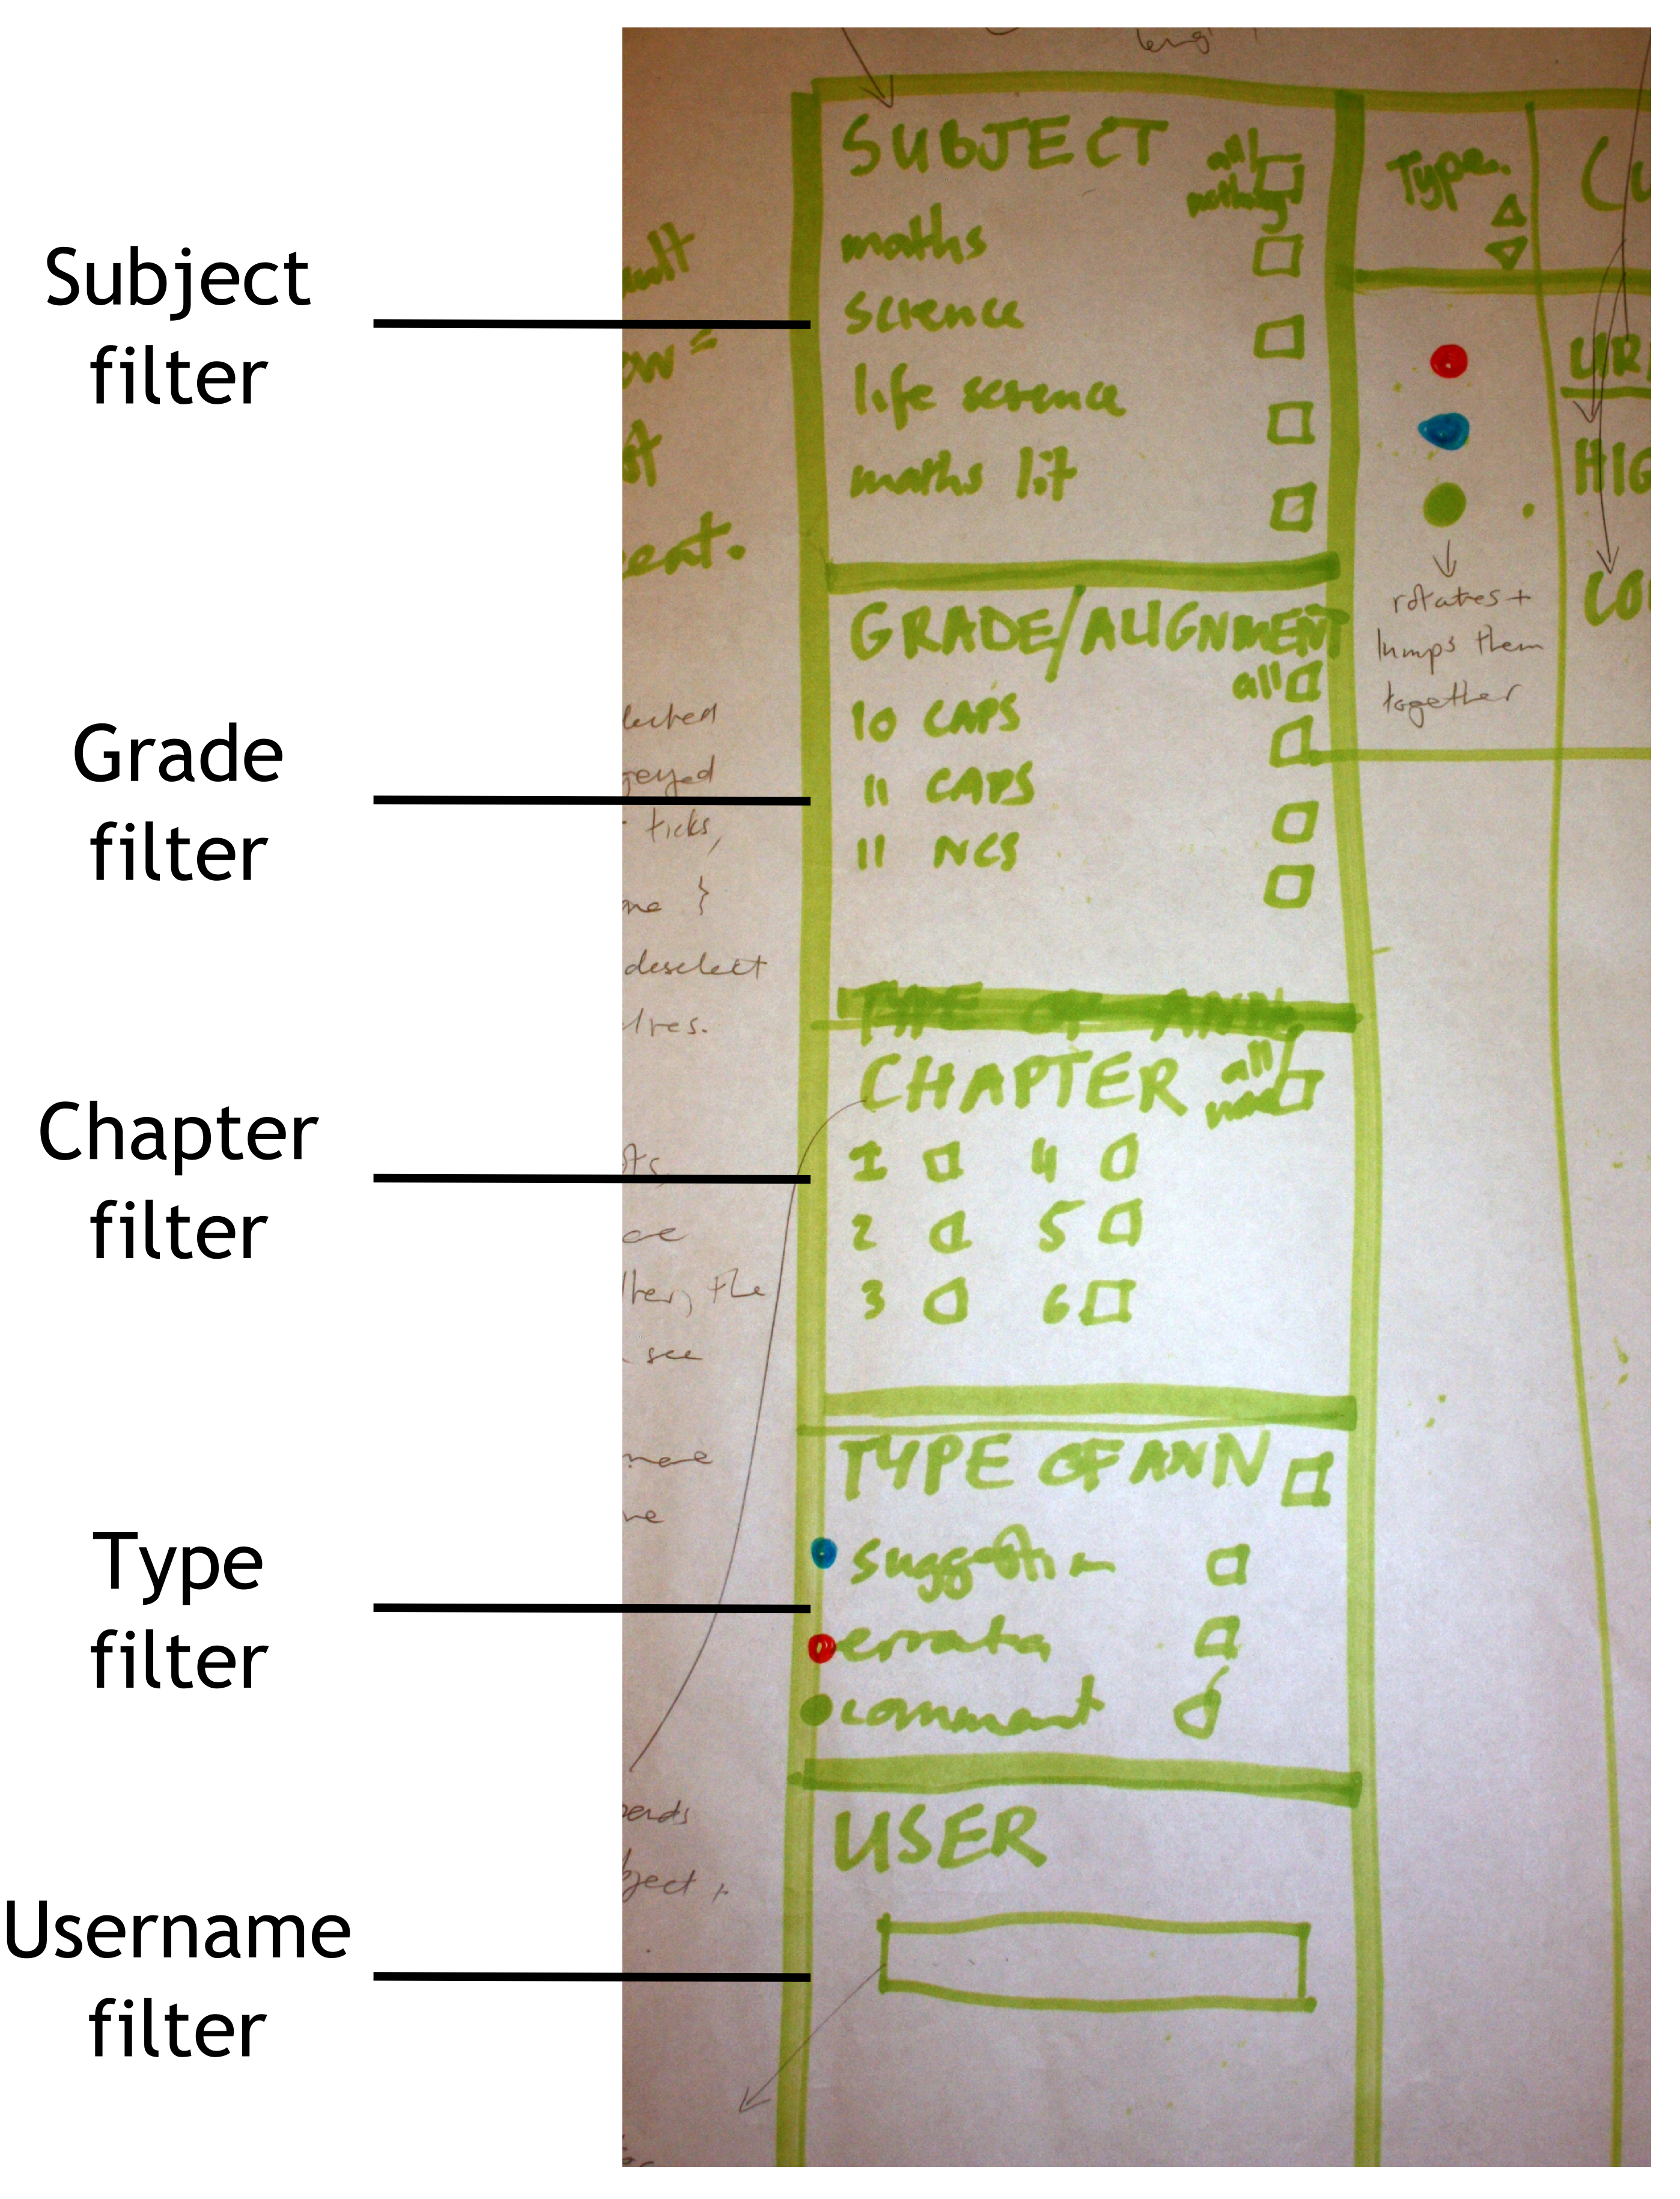
\includegraphics[width=0.6\textwidth]{Figures/PDfiltersLabels.png}
 \caption{Filter boxes in the final paper prototype.}
 \label{fig:FilterBoxes}
\end{figure}

The basic behaviour is that the user would initially see all the available annotations, and that ``the more they click, the less they see". So selecting filter options would refine the results displayed (live) in the table on the right. 

As mentioned above, the username search box would function like an autocomplete search, querying the database of known usernames as a user starts typing. A ``Reset" or ``Clear" button (Label 6 in Figure \ref{fig:FinalPP}) would be placed at the bottom of the left-hand options to return the displayed results to the default view. 

The table of displayed results would have the following sortable columns (see Figure \ref{fig:TableHead}): \\
$\vert$ Type $\vert$ Info (URL, comment \& highlighted text previews) $\vert$ Number of replies $\vert$ Date $\vert$\\
\\
\begin{figure}[h!]
    \centering
    \includegraphics[width=\textwidth]{Figures/PDColumnHeadingLabels.jpg}
 \caption{Table heading columns in the final paper prototype.}
 \label{fig:TableHead}
\end{figure}
The default sort would be by date, with the most recent annotations listed first. The URL would hyperlink to the actual annotation in the book and the ``Info" column would be sortable by URL (which corresponds to books and their chapters and sections). Breadcrumbs like $\vert$ Previous $\vert$ Next $\vert$ 20 $\vert$ 50 $\vert$ 100 $\vert$ would occur at the bottom of the table of results. 

The type of annotation would be indicated in the leftmost column by a small coloured icon. This column would sort in a rotational manner. 

Clicking on a particular annotation would open a detailed view of said annotation in a window (or frame) in the same page. Right-clicking a particular annotation would allow the user to open it in a new tab. This detailed view would contain all the available information about the annotation (full URL, comment, highlighted text, username, date, replies), and the hyperlinked URL to take one quickly to the original annotation in the context of a book.
\begin{figure}[h!]
    \centering
    \includegraphics[width=\textwidth]{Figures/IMG_9044.JPG}
 \caption{Detailed view overlay in the final paper prototype, showing more information for a specific annotation.}
\end{figure}
Clicking ``Back" from the detailed view would take users back to their previous set of filters and results. Likewise, if a user logged out and in again, or navigated back to the back-end interface from another page, they would see their last search results. 

\section{Discussion}
Overall, the participatory design process was very constructive and informative. It was extremely valuable to get user input, and having participants work in a group together meant that they could discuss and refine ideas with each other and reach a unified design concept which satisfied everyone. 

Drawing several iterative sketches of the interface enabled participants to explore and experiment with different possibilities together. These sketches also seemed to help participants visualise concepts and explain ideas to each other. Whilst some participants were more comfortable talking than drawing, the group struck a balance between thinking out loud and visualizing their ideas on paper for others to see.

Many ideas were brainstormed and then included or discarded as the participants' design evolved. These included different filter options (e.g. the keyword search, which was discarded later on), layout options (participants experimented with dropdown filters before they decided on the left column layout), table heading options and assorted interface behaviours (e.g initially paritipants suggested collapsible filter sections, but later discarded this idea once they'd narrowed down the list of filter options and determined that they could probably all fit in the same view even if they were expanded).  

Because participants were used to brainstorming processes in the workplace, they were generally open to each other's suggestions and criticisms and there was little discrepancy between participants ideas and suggestions, with the exception of the issue tracking question. 

Having two separate sessions spaced one week apart also gave participants an opportunity to mull over ideas that had been discussed before the second session. 

Sometimes the brainstorming became very creative and extended beyond the scope of the interface in question. In these instances it  was challenging to try and keep participants focused on the task at hand, without dampening their enthusiasm. 

While the paper prototype seemed like a viable design solution that would thoroughly address user requirements, ultimately any proposed functionality that required issue tracking integration (e.g. GitHub) or server-side processing had to be excluded. This was in order to limit the scope of the project slightly and focus on the interface functionality itself, instead of the design of a database system that would have to include user authentication, server integration and so on. 
 
% Chapter 6

\chapter{Building a High-fidelity Prototype} % Main chapter title

\label{Building a High-fidelity Prototype} % For referencing the chapter elsewhere, use \ref{Chapter1} 

\lhead{Chapter 6. \emph{Building a High-fidelity Prototype}} % This is for the header on each page - perhaps a shortened title

%----------------------------------------------------------------------------------------

Once the paper prototype was complete, it was converted into a Balsamiq \citep{Balsamiq} mockup (see Figure  \ref{fig:Balsamiq}), to be as tidy and legible as possible, as well as digitally portable. This allowed for easy sharing and backing up (e.g. it could be saved to Dropbox and viewed anywhere, on any device) because it was a small PDF file and not an A2 roll of paper. It also provided a more legible version of the paper prototype that didn't include scratched out notes or other visual ambiguities that could confuse the development process. 

%\begin{figure}[h!]
\begin{sidewaysfigure}
    \centering
    \includegraphics[width=\textwidth]{Figures/BalsamiqMockup.png}
 \caption{Balsamiq mockup of the final paper prototype.}
 \label{fig:Balsamiq}
 \end{sidewaysfigure}
%\end{figure}

This mockup was then converted into a functional, high-fidelity prototype website using HTML, CSS and XML, as is detailed below. Scripted functionality was built using Javascript and the JQuery library in particular.  

The site was hosted using GitHub Pages \citep{GitHub} at \href{http://nicoladt.github.io/MIT-Thesis/}{http://nicoladt.github.io/MIT-Thesis/} which offers simple, free hosting, and seamless integration with GitHub version control software. Assistance was given by Ewald Zietsman with the Javascript and JQuery coding. 

\section{The high-fidelity prototype}



\subsection{Technical details}
The interface was comprised of two main areas (see Figure \ref{fig:HifiMain}). The column on the left contained all the filter options, and the table making up the rest of the page displays the annotations in rows.

Placeholder annotations were made in an XML file. Each annotation was assigned a type and had a simple data structure including a timestamp, a URL (pointing to a particular webpage on the live webbooks sites), a username, highlighted text (from the book), and a user comment. In addition each annotation could have one or more replies. Replies in turn also had a timestamp, username and user comment: 
\begin{verbatim}
<annotation type="">
  <url></url>
  <username></username>
  <datetime></datetime>
  <highlighted></highlighted>
  <comment></comment>
  <replies>
    <reply>
      <username></username>
      <comment></comment>
      <datetime></datetime>
    </reply>
  </replies>
</annotation>
\end{verbatim}

For the prototype, annotations were not given unique ID's or primary keys. Whilst this would be necessary for real annotations (due the the possible complexities of many users making many annotations simultaneously), for the prototype a combination of the URL and timestamp was used as a unique identifying characteristic. 

Annotations were constructed carefully with evaluation tasks in mind. They were created so as to represent at least every possible combination of subject and grade. Annotations were assigned to the three types (comment, errata, suggestion) and random usernames were created. Replies (in number from 1 to 3) were added to some annotations.

The interface was built upon the basic components of the Bootstrap 2.3.2 framework \citep{Bootstrap}. Bootstrap was selected not only because of its built-in cross-browser compatibility but also because it comes packaged with clean and simple CSS and a number of default elements (like buttons) that are easily customizable. 

The DataTables jQuery plugin \citep{DataTables} was implemented for easy control over the table and its functionality and behaviour. 

%\begin{figure}[h!]
\begin{sidewaysfigure}
    \centering
    \includegraphics[width=\textwidth]{Figures/V1/HiFi1mainview.PNG}
 \caption{Screenshot of the high-fidelity prototype.}
 \label{fig:HifiMain}
\end{sidewaysfigure}
% \end{figure}

A fixed header for the the table was deemed important, so that users always knew what each column represented. However, DataTables fixed header functionality does not work correctly with pagination (a known bug), so a compromise was reached and vertical scrolling was enabled instead. Pagination breadcrumbs (arguably not necessary for sets of annotations $<$ 100 entries) beneath the table, were substituted with the automatically-updated line of text saying "\textit{Showing xx number of yy entries}", where xx was the number of rows in the table, and yy the total number of annotations (see Figure \ref{fig:breadcrumbs}).

\begin{figure}[h!]
    \centering
    \includegraphics[width=0.7\textwidth]{Figures/V1/breadcrumbs.png}
 \caption{Text beneath the table indicated how many rows (annotations) are surfaced}
 \label{fig:breadcrumbs}
\end{figure}

DataTables also contains an unfortunate (and well-documented) CSS bug, in which the fixed table header \verb|<th>|                                                                                                                cells do not always align correctly with the table data \verb|<td>| cells beneath them. However, this is a minor visual issue concerning a few pixels.

DataTables can only handle an alphabetical sort of columns, which meant that a three-way (rotational) sort of the "type" column was not possible - i.e. it was not possible to sort so that "errata" was listed at the top, "e" being between "c" (comment) and "s" (suggestion) in the alphabet. Additionally, it is only possible to perform a default sort on one column initially, so a sort based on Date and then Type was not possible.

Whilst the loss of these possibilities is noteworthy, it was decided to proceed with the implementation of the DataTables plugin, because the missing functionality could easily be substituted using other techniques (e.g. it was very easy to filter all the annotations by "type" to get to the third sorting category of "errata"). For this reason it was decided that the pros of using the DataTables plugin outweighed these few cons.

Javascript and the jQuery library were chosen to do the information processing required by the interface. jQuery allows for client-side processing. It is simple to implement, and runs as a light-weight instance in any browser \citep{jQuery} \citep{JS}. Practically, client-side data processing (as opposed to HTTP calls to a server) allows for rapid updates to a webpage, and therefore to the interface itself. 

GitHub Pages was selected as the simplest hosting solution for the prototype, because it is secure and reliable, and most-importantly integrates seamlessly with GitHub version control software. However GitHub Pages can only serve static HTML and it cannot handle server calls. Again, the pros of using GitHub Pages outweighed the single loss of functionality it presented, which was the inability to use cookies to store user session information. 


In terms of scripting behaviour, the script written parses the list of XML annotations and builds then builds the filters on the left of the interface based on what it finds in the XML. Each URL from everythingmaths.co.za and everythingscience.co.za contains information about the subject, grade, chapter and section applicable to that annotation. This information is parsed from the URL and presented in a human-readable text format, both as filters on the left-hand side, and as inline text for each annotation. 

\subsection{Behaviour}
Once the filters have been constructed from the XML, the table is then populated based on  the selection filters on the left of the page. The default is that all the annotations are selected and therefore all the annotations are displayed in the table. The basic behavioural pattern is that interacting with the left-hand filters automatically changes what is visible in the table. Any changes made to the left-hand selection cause the table to display only the annotations relevant to the new parameters selected on the left. 

The checkboxes are grouped according to the field \citep[p. 439]{Galitz}: i.e. by subject, grade, chapter number and type. 

Initially the 'All' checkboxes were ticked, and the sub-checkboxes were also ticked but greyed-out, as per the paper prototype. Clicking on a sub-check selected that particular checkbox, deselected the "All" checkboxes and deselected all other sub-checkboxes. It also made the sub-checkboxes opaque (see Figure \ref{fig:checkboxes1}). 

\begin{figure}[h!]
    \centering
    \includegraphics[width=0.4\textwidth]{Figures/V1/checkboxes.png}
 \caption{Single selection of sub-checkbox, compared to selection of "All" checkbox.}
 \label{fig:checkboxes1}
\end{figure}

Clicking on an checked "All" checkbox deselected the "All", selected all of the sub-checkboxes in that filter category, and made them opaque (see Figure \ref{fig:checkboxes2}). In other words, the "All" checkbox behaved as an 'all or subset' toggle, not an 'all or nothing' toggle (which would just result an empty table). 

Whilst this deviated from the standard checkbox behaviour ('all or nothing'), firstly it is the behaviour participants suggested in the design sessions. Secondly \citep[p. 435]{Galitz} this modification allowed for the possibility that a user would want to invert a selection: i.e. to select most (but not all) of the sub-checkboxes in a category. For instance, a user might want to select 23 of of 24 chapter checkboxes. Clicking 23 times would be tedious indeed. With the "All" behaviour described above, a user could simply deselect the "All" checkbox and deselect the chapters they did not want included in the results.

\begin{figure}[h!]
    \centering
    \includegraphics[width=0.3\textwidth]{Figures/V1/alldeselected1.PNG}
 \caption{Subject, with "All" checked vs. Grade, with "All" unchecked and all sub-checkboxes activated.}
 \label{fig:checkboxes2}
\end{figure}

The username search box was a simple, case-sensitive text search. It did not serve up an auto-completing drop-down list. Instead, the table updated automatically (with each new character typed) as the user began typing into the input box. This alternative behaviour to that specified in the paper prototype was selected because it was consistent \citep[p. 261]{DixFinlay} with the behaviour of the table for all other filter fields, whilst still giving users the immediate feedback they required (in the form of instantly updated results with every keystroke) when performing a potentially uncertain search for a username. 

The button labelled "Reset" simply reset the page to the default view (see Figure \ref{fig:reset}). 
\begin{figure}[h!]
    \centering
    \includegraphics[width=0.4\textwidth]{Figures/V1/usernameReset.png}
 \caption{The username search box and "Reset" button.}
 \label{fig:reset}

\end{figure}

The table was sorted by default by descending date (see Figure \ref{fig:sort}).  As mentioned above, it was not sorted with errata at the top of  the type column due to DataTables' strictly alphanumeric sorting capabilities. That being said, an alternative method for viewing "errata" type annotations at the top of the table was provided by the type filter on the left so this was deemed an acceptable alternative. 
\begin{figure}[h!]
    \centering
    \includegraphics[width=0.35\textwidth]{Figures/V1/sorticons.png}
 \caption{"Sortable" vs "sorted: descending" icons in the table header}
 \label{fig:sort}

\end{figure}	

On mouseover of the table rows, the row changed colour (from white to light grey) and the cursor changed to be a "zoom in" cursor to indicate that action is possible: that the row is clickable and there are more details to be viewed or expanded (see Figure \ref{fig:mouseover}).

\begin{figure}[h!]
    \centering
    \includegraphics[width=\textwidth]{Figures/V1/mouseover.png}
 \caption{Grey row colour and zoom icon on hover.}
 \label{fig:mouseover}

\end{figure}

Clicking on a particular annotation brought up the detailed view window as an overlay on the table (see Figure \ref{fig:detailedview}). As well as all of the annotation information visible in the table, this view also included all replies to an annotation and the reply details. To close the detailed window, users could click on the [x] in the top right corner of the window or they can press the [Esc] key. 

Because the detailed view was an overlay of the interface and not a separate browser window, a "Back" button (as in the paper prototype) was not included. Users were given two standard alternatives to close the overlay instead. 

\begin{figure}[h!]
    \centering
    \includegraphics[width=\textwidth]{Figures/V1/detailedview.png}
 \caption{The detailed view overlay.}
 \label{fig:detailedview}

\end{figure}

\section{How and why the high-fidelity prototype differs from the paper prototype}
As mentioned in Chapter 5, certain functionality that was discussed in the paper prototyping process was excluded because it required the integration of server-side processing and issue tracking software, which would significantly extend the scope of the system. Differences between the paper and high-fidelity prototypes are detailed as follows. 
\begin{enumerate}
 \item \textbf{No cookies}\\
For simplicity of development and in order to use GitHub Pages for hosting, the interface only used client-side processing, without any server integration. This meant that cookies to store information about a user's session could not be saved and that if a user navigated away from, and back to the webpage, it would be reset to its default view: the user's last filter selection would not be saved. \\
\\
The advantages gained by using GitHub were significant, as mentioned already. Additionally, it could be argued that the selection of filters and live updating of the resulting table was simple and quick enough that redoing a task would be relatively trivial. 

\item \textbf{No user authentication}\\
Again, because of the lack of a server, user authentication was not implemented in this prototype. Authentication is arguably not needed to test the interface functionality itself however: it would be an independent process that would take place in its entirety before a user came to view the interface in question. 

\item \textbf{No collapsible filters}\\
The groups of filters and checkboxes were not collapsible, because they all fitted onto one page. The collapsibility was suggested by users during the paper prototyping sessions because they were concerned that there would be too much information to fit onto one webpage. In implementation however, this was not the case, so this functionality was set aside. Because the filters offer a graphical representation of the system status (what is visibly selected on the left maps directly to what information is in the table) displaying all filters on one page also improved observability \citep[p. 270]{DixFinlay} for users.

\item \textbf{No username auto-complete suggestions}\\
The username search box did not offer a drop-down list of auto-complete suggestions when users started typing. Instead, it updated the table of results automatically with each keystroke. This behaviour was the same as for all the other filter categories, and so it replicated a pattern found throughout the interface (consistency and predictability), while still giving users immediate feedback (instantaneous responsiveness) and the easy ability to undo actions (recoverability) \citep[p. 272]{DixFinlay}. 

\item \textbf{Extra information added to each annotation cell}\\
At the top of each "Annotation Info" cell, a line of bold text containing the subject, grade, chapter number and chapter name was added to give users more  easily readable information about where each annotation was from, so they did not have to decipher a long URL.

\item \textbf{No back button in detailed view}\\
Because the detailed view was an overlay and not a new webpage a "Back" button was not included (users making the prototype specified that the detailed view should open in the same page). Instead, users could close the overlay by clicking on the [x], in the top right corner, or by pressing the [Esc] key - both standard interface patterns \citep[p. 345]{Galitz}. Using an overlay instead of a new webpage or window also prevented users from leaving the webpage unnecessarily, and therefore reduced the risk of users getting lost in a navigation process. 

\item \textbf{No Life Sciences subject}\\
Due to external factors, the Life Sciences Grade 10 book was not yet available on the Everything Science website, so it was excluded because there were no live URLs available for that content. 

\item \textbf{No curriculum alignment filter}\\
By the time the high-fidelity prototype was being built, all available textbooks on the Everything Maths and Science websites were aligned to the current CAPS curriculum, and no old NCS content was available. Hence, the curriculum alignment filter was excluded. 

\item \textbf{Lower-level filters do not update}\\
Participants in the design sessions suggested that lower-level filters (like chapter) should update based on the higher selection. I.e. the list of grade filters would update depending on the subject choice, and the number of chapters would change to reflect what was available in a specific combination of grade and subject. \\
\\
If users performed a unidirectional filter operation this functionality would be useful. However excluding it and displaying all possible subjects, grades and chapters meant that users could easily change their selection, and filter both forwards and backwards. This made it far simpler to correct mistakes, undo actions or browse the data and discover new information, all of which conforms to good design principles \citep[p. 272]{DixFinlay}. \\
\\
Additionally, displaying all of the possible filters at once meant that users always have visual feedback about what they \textit{had} selected, in the context of what they \textit{could} select. This would make current and future states more apparent and discoverable (which ties into the design principle of observability \citep[p. 270]{DixFinlay}).  

\item \textbf{No coloured dots next to "Type"}\\
The coloured circle icons suggested for "Type" categories were replaced by coloured labels beneath the "Type" text.  These coloured labels are packaged as part of the default Bootstrap styles, and were therefore simplest to implement, the visual  effect arguably being the same. Three colours were selected based on users' paper prototype suggestions, available Bootstrap label colours and common meanings for colour \citep[p. 635]{Galitz} (e.g. red, which often signifies a warning was used for errata).

\item \textbf{No right-clicking of rows}\\
Right-clicking an annotation row did not open it in new tab. This was simply because the detailed view was constructed as a visual overlay, and not as a new webpage. 

\item \textbf{DataTables-related changes}
  \begin{enumerate}
    \item \textbf{No double default sort}\\
    As discussed above, using DataTables meant that it was not possible to perform a default sort by date \textit{and} type. Because of the ease with which users could filter by type on the left-hand side of the interface, the default sort was simply by date, descending. 
    \item \textbf{No breadcrumbs or pagination}\\
    Due to DataTables' fixed table header not working with the built-in pagination functionality, pagination was substituted with vertical scrolling. Instead of "Previous $\vert$ Next $\vert$ 10 $\vert$ 20 $\vert$ 50 $\vert$" breadcrumbs at the bottom a message was surfaced indicating how many annotations (rows) were displayed in the current table.
    \item \textbf{Strict alphanumeric sorts}\\
    Because DataTables' sorting functionality is strictly alphabetical, a three-way sort for the type column (to surface "errata" at the top) was not possible. Similarly, the annotation information column could not be sorted by URL. Instead it was sorted by the subject, grade and chapter number text at the top of each cell (the same information that the URL provided anyway). 
  \end{enumerate}
  
\end{enumerate}

\section{Discussion}
Whilst the high-fidelity prototype did diverge from the paper prototype slightly, wherever possible behaviour or design specified in the paper prototype that could not be included was substituted with an equivalent solution. Trade-offs (e.g. using DataTables) were carefully evaluated so that whenever possible, more functionality was gained than was lost or had to be altered. 

Any divergence could (and would) also be thoroughly evaluated by users in the next part of the process, involving usability testing and formative evaluation. 

In some cases, the implementation of the prototype in an actual web browser opened up new possibilities - such as styling the filters to all fit on one standard 1366 x 768 resolution screen. The visual effects of an overlay are also easier to envision and explore with HTML and CSS than on paper. 

Several aspects of the high-fidelity prototype were not highly scalable. For example, client-side processing of thousands (not dozens) of annotations in future would get extremely slow. Similarly, while reloading the table with a few annotations takes only milliseconds, with a large database of annotations, and a more complex set of filters (e.g. more subjects, more grades) the load time would be significantly increased. There is no doubt a performance threshold at which it would become practical to implement server-side processing instead, which would also mean that user authentication and use of cookies would become possible. Similarly, with a larger database, pagination of the table (with breadcrumbs) as opposed to vertical scrolling would be necessary to reduce load and response time of the interface. 

Whilst DataTables provided a lot of pre-packaged functionality, it is currently not very robust, and it appears that new releases and improvements, while pending, are slow to occur. Ideally it would be better to reinvent the wheel, and write customised code to handle sorting (e.g. three way sort, implementing more than one default sort parameter), pagination, header behaviour and so on. 

Once the high-fidelity prototype of the interface was complete the next step was to formatively evaluate it with a new group of users \citep[p. 329]{RogersPreece}, to ensure that the design thus far still conformed to user requirements and expectations. Once this was done, the interface could then be iteratively improved based on the first round of usability tests and user feedback. This process of evaluation and iteration will be discussed at length in the next chapter. 
 
\part{Evaluation and Improvements}
% Chapter 7

\chapter{Evaluation and Improvements} % Main chapter title

\label{Evaluation and Improvements} % For referencing the chapter elsewhere, use \ref{Chapter1} 

\lhead{Chapter 7. \emph{Evaluation and Improvements}} % This is for the header on each page - perhaps a shortened title

%----------------------------------------------------------------------------------------


\section{Formative evaluation}
Formative evaluation is evaluation that takes place during the design process and is used to improve a design citep[p. 149]{Hartson}. It focuses on identifying usability problems in a prototype that should and can be addressed during an iterative design process. It also ensures that users continue to be included in development, because their feedback is central to improving the design \citep{GabbardHix}. 

The goal of the formative evaluation process was firstly to determine that the high-fidelity prototype was an accurate representation of the paper prototype, according to the users' conceptual models, and secondly to establish that the interface met the high-level user requirements determined earlier in the design process.

Following the process outlined by Gabbard et al  \citep{GabbardHix}, user questions and tasks were developed to test all functionality and behaviour of the interface. In particular, the tasks were designed to test the user requirements that emerged from the requirements analysis process and the paper prototyping sessions. The test was practised informally (with a willing family member) before users were involved, to ensure that the wording of questions and tasks made sense and that the evaluator was comfortable with the test material.

Users were first asked interview-type questions to assess their conceptual interpretation of the interface. Without interacting with the system (they could move the mouse and hover over elements, but not click on anything), users were asked what they thought various visual elements represented, and how they would expect them to behave were they to interact with them. These questions were designed to determine initial user expectations and assumptions, and were phrased such as ``\textit{what do you think xx represents?}" and ``\textit{what would you expect to happen if you clicked on yy?}". 

Users were then asked to complete the tasks (with free reign of the mouse or keyboard), which were contextualised with reality-based scenarios.

The test questions are documented as follows.

\textbf{To test interface components:}
\begin{enumerate}
 \item What do you think the left hand area of the page represents?
 \item What do you think will happen if you interact with anything the left hand side of the page?
  \item What do you think the rows in the table represent?
  \item What do you think each group of checkboxes represents? 
   \begin{enumerate}
    \item What do you think will happen if you click on an ``All" checkbox?
    \item Do you think the greyed out checkboxes are clickable? If so, what do you expect to happen if you clicked on one of them?
   \end{enumerate}
  \item What do you think the text box beneath the checkboxes is for?
  \item What do you expect will happen if you start typing into that box?
  \item What do you think the button labelled ``Reset" does?
  \item What do you think the zoom cursor on mouseover means?
  \item Do you think the rows are clickable? If so, what do you think would happen if you clicked on a row?
  \item In the column called ``Annotation information", what do the four bold pieces of text at the top of each cell refer to?
  \item What do you think the little arrows in the top row of the table mean?
  \item Do you think the table is sorted by default? If so, why do you think so? And how do you think it's sorted? 
\end{enumerate}

\textbf{To test interface behaviour:}
\begin{enumerate}
 \item Let's say you've been asked to find all annotations made in Physical Sciences. What would you click on?
 \item Without using your mouse, how many annotations do you think there there? How do you know this?
 \item Say you want to refine your search to all annotations in Physical Sciences, Grade 10. What would you click on?
 \item Next, what if you want to refine your search to all annotations in Physical Sciences, Grade 10, Chapter 5. What would you click on?
 \item Let's assume you've found the annotation you were looking for. and now you'd like to clear your search thus far, and return to the initial view of the page. What would you click on or do to achieve this? (To reload the page/reset to defaults.)
 \item If you'd like to find all annotations that users have labeled as being comments. What would you click on?
 \item Let's say a user calls the office to ask if his annotation has been captured in the system. His username is ``bob" (all lowercase). You need to find all the annotations by this user. What would you do first?
 \item If you need to find all annotations made by users with usernames starting with lowercase ``s", what would you do?
 \item Let's say you're not sure about a user's comment and would like to view the original webpage where the webbook text was annotated. How would you go about this?
 \item What if you'd like to view all suggestion type annotations at the top of the table:  what would you do to sort them? 
 \item Let's say you need to find the annotation with the highest number of replies. What would you do to find this?
 \item You'd like to know more about the annotation with the highest number of replies. What would you do [if anything] to find more information about this annotation and its replies? 
 \begin{enumerate}
 \item  What text do you think was annotated by the original user? [Assuming user clicks on an annotation]
 \item Who do you think was the original user? Why do you think this?
 \item What do you think the original user's comment on the text was? Why do you think this?
 \item Which user replied do you think first to the original annotation, and when did they do it? Why do you think this?
 \item What do you think that user's reply was? Why do you think this?
 \item If you'd like to go back to the main page/view. what would you do?
 \end{enumerate}
 \item Let's say you need to check that there aren't any annotations in subjects other than Maths, Maths Lit or Physical Sciences (e.g. Biology). How would you go about this? What would you click on first?
 \item Let's say that you've been asked to check that no annotations have mistakenly been made under Maths Lit Grade 11. How would you go about doing this? What would you click on first? 
 \end{enumerate}
 

\subsection{Usability test results}
\underline{User A} thought that the greyed out sub-checkboxes did not look clickable. He also thought that the username search box looked greyed out. He was uncertain as to how the username search box would behave: while he noticed there was no ``Search" button to submit a user search he did not know if the search box would ``\textit{filter on the fly}" or offer an autocomplete dropdown list of matching usernames. He said it was not always obvious that the table rows had actually updated when he had interacted with a filter.

He realised that the zoom icon (when hovering on a table row) indicated expansion, but was not sure what information an expanded view would include. He commented that the cursor did not change if he hovered over the table header sort icons, so it did not seem clear that the sort arrows were clickable because: ``\textit{When you can click on things you get the finger}" (\includegraphics[width=0.5cm]{Figures/handcursor.png}). He also noticed that when hovering over the table header text (e.g. ``Type") the cursor changed to be a text input cursor (\includegraphics[width=0.5cm]{Figures/textcursor.png}). This was a default DataTables/Browser behaviour which the evaluator had not noticed in testing before.

In addition, User A noticed the DataTables CSS bug already mentioned, where in some instances the fixed table header cells do not align correctly with the table data cells in the rows beneath them.

To close the detailed view overlay, he tried clicking off the box, which did not work - he felt it ``\textit{probably should}". He also mentioned that he thought the Reset button was ``\textit{a bit obscured}" at the bottom of the page, and suggested renaming it to ``Reset Filters" and moving it to the top of the page. 

\underline{User B} also did not think that the greyed out sub-checkboxes were clickable - she assumed they would become clickable if she unchecked ``All". She also expected the ``All" checkbox to be an all/none toggle, so that if ``All" was unchecked, then nothing would be selected. When she realised this was not the case (unchecking an ``All" selected all the sub-checkboxes instead), she deselected the sub-checkboxes to get to the required filter set. For example, to select the ``chapter 5" filter - she unchecked the ``All", which selected the 24 sub-checkboxes for ``Chapter" and proceeded to deselect 23 checkboxes until just ``5" was selected. Even though she realised this was inefficient and unlikely to be the only solution, she did not experiment with the checkbox behaviour to see if an alternative option was available. 

The purpose of the username search box was not initially clear to her as she did not know what it would be used to search for. She also was not sure how it would behave and whether she would have to press ``Enter" to submit a search, for example. Once she interacted with the search box however, she realised that it filtered the table automatically. 

User B also missed the visual indication of the default date sort (\includegraphics[width=0.3cm]{Figures/sortarrowdown.png}). She realised the table was sorted by date, but she deduced this from the date column entries.

\underline{User C} did assume that the greyed out sub-checkboxes were clickable. However, when she interacted with the system, she first tried to deselect one, and then discovered that clicking on one actually selected it. However, she did not think to deselect all subject checkboxes to get no results in the table. 

She did not expect anything to happen if she started typing in the username search box, and she mistook the ``Reset" button for a username ``Search" (submit) button: she assumed she would have to type in the box and then press ``Reset" to submit her user search. 

When she started interacting with the interface it was apparent that her confusion about the ``Reset" button extended beyond this: after she selected the relevant group of checkboxes to a particular task she clicked the ``Reset" button to submit her entire filter query (i.e. she did not notice the table updating at all) and then was perplexed when she realised her filter choice had just been cleared. According to her: ``\textit{I would want to choose something and then click something else.  It would make sense if you had some instructions. I think it's important to have a Reset button because there's quite a lot of options… But my initial thing is that you choose and click Enter [to] search. That's how you do it on Google}". 

User C thought that the zoom icon on row mouseover meant that the rows were clickable, but was not sure what clicking on a row would do (``\textit{either it would bring up more information, or single out that particular comment but I don't know how...}"). Eventually we established that she expected the zoom icon to indicate a literal, visual zooming in, i.e. making the text bigger (``\textit{why would you want to see it bigger, when you can read it?}"). She did not think that clicking on a row would bring up more detailed information and she only noticed that the URL in each row was clickable. 

She was uncertain as to how the ``Annotation Information" column would sort itself, and was not sure why one would want to sort the table by ``Type", when ``\textit{you can do that with the filters on the left}". When she initially clicked on a sort icon, the table update was not obvious (the sorting change to the visible results was minimal), and this confused her. However she persevered and clicked again, and then realised that the table had updated. 

She thought that the coloured type labels looked like clickable buttons. She also noticed a bug where, even when there were no entries in the table, the counter text at the bottom still displayed ``Showing 1 of 1 entries".

\underline{User D} did not think that the greyed out sub-checkboxes were clickable in their initial state but thought they probably would be if the ``All" checkbox was deselected (i.e. an all/some toggle). That being said, initially she did not try to click on a greyed out sub-checkbox - she deselected ``All" first and then clicked on a (already checked) sub-checkbox. She realised that deselected the sub-checkbox. She experimented and discovered by accident that she could just select one greyed out sub-checkbox directly. (For the chapter selection task where she discovered this alternative behaviour she said: ``\textit{I wasn't going to uncheck them} [23 chapter numbers] \textit{all!}"). Interestingly, even after she realised she could just directly select a greyed out sub-checkbox, for the next tasks she went to uncheck ``All" again, first. Like User C, she did not think to deselect all subjects to get no results in the table. 

User D thought that the username search box was for ``\textit{your username}" (i.e. that one would input your own username into the box, and that it was not a search). She did not expect typing in it to have any effect on the table. Then, in one task, she typed the text ``Comment" in the box, to search for it. Based on this experiment, she then realised that the search box was specific, not general (i.e. not a site search), and then understood that it was to search for usernames in the table. In a later task, when she searched for ``s" in the username search box, the table updated so fast that she initially did not notice the results had changed.

She did not know what the sorting arrows in the table header indicated, and did not notice the Date default sort icon. She did not think that it was possible to sort by a column header until she tried clicking on the ``Replies" header. When asked to sort by the highest number of replies she said: ``\textit{I'd try and click here somewhere… [clicked] ``Oh and that's what it does!}". She also noticed that the date sort, which at first glance looked correct, was in fact not (caused by a bug in the code that converted a long timestamp into human-readable text). 

User D did also not believe that the zoom icon indicated that the row was clickable. For her, it was not obvious that she could click on a row, or that doing so would surface additional details about that row. 

\underline{User E} initially thought that deselecting an ``All" checkbox would result in one of the sub-checkboxes being selected. She did not think that the greyed out sub-checkboxes were clickable, but said that the changing mouseover icon suggested that they were. She expected to have to uncheck the ``All" checkbox first. When she actually interacted with the interface however, she tried clicking directly on a greyed out sub-checkbox (without deselecting the ``All") and realised that was possible. Despite this, she said ``\textit{my instinct is still to uncheck 'All' first and then click on the others}".

With respect to the username search box, User E said that she hoped the table would not update until she had finish typing a username into the search box, because she was concerned that it would be very slow. She thought the search box might offer a dropdown list of autocomplete options, and said that that ``\textit{would be good}". She initially assumed that she would need to hit ``Enter" to submit her search, but then noticed that there was no ``Search" button, so she assumed the search box must filter the table automatically. In a later task when she actually interacted with the search box, she noticed that it updated automatically as she typed. 

Like User A, User E said that she expected the cursor to change when she moused over the sort icons in the table header. She noticed that a three way sort was not possible and that she could not sort to have the ``Errata" type at the top of the table. ``\textit{It only has two...Then again I could just click on Errata [in the type filter on the left] if I just wanted them}". She suggested the text ``asc" and ``desc" instead of just the sorting arrows - she felt that the arrows alone were too visually subtle. She also was not sure how the ``Annotation Information" column would be sorted. 

For the detailed view overlay, like User A, she tried to click off the detailed view box to close it, which did not work. She also suggested using a ``zoom out" icon when in the detailed view, to ``\textit{match the zoom in icon}" which opened the detailed view in the first place. 

The above feedback can be summarised as follows:
\begin{itemize}
\item It was apparent that the behaviour of the checkboxes was not immediately obvious to users and that this needed to be reevaluated. 
\item Additionally, the table often updated too quickly for users to notice that it had changed. 
\item The cursor icons on hover needed to be changed, to make it very clear where and when users could click on things (e.g. on the sort arrows but not on the header text). 
\item The sort arrows were not visually obvious enough.
\item The purpose of the Reset button was not immediately apparent, and users got confused as to whether or not it was related to the username search box. 
\item The purpose of the username search box was not clear enough, and users did not expect the automatic updating behaviour (of the table) associated with the search box. 
\item Users expected to be able to click off the detailed view to close the overlay. 
\end{itemize}
In addition, the evaluator also noticed a number of bugs and issues with the interface during the usability tests:
\begin{itemize}
\item A possible fix for the DataTables CSS \verb|<th>| bug needed to be investigated: at least one user noticed it and commented on the fact the the table header did not always line up.
 \item It was observed that clicking on the URL in a row triggered the OnClick event to open the detailed view. So, if a user clicked on the URL, the detailed view would open, and only then would the user be taken to the relevant Everything Maths/Science webpage. This needed to be fixed. 
\item It was also noticed that if a user had searched for a username, navigated away from the web page (e.g. to the Everything Maths/Science URL) and hit ``Back" in the browser to return to the interface, the filters would all be reset on the page but the last string the user had searched for would still be visible in the username search box, which was misleading. 
\item It was noted that the numeric date sort did not work correctly because of the order in which the date components (year, month etc) were parsed by the JavaScript. 
\item It was also noted that not one user pressed the [Esc] key to exit the detailed view. 
\end{itemize}

\section{Improvements to the prototype}
Based on the above observations, improvements to the prototype were implemented as is detailed in the following sections. Due to the very small sample size, no meaningful statistical analysis could be performed on the test data \citep[p. 149]{Hartson}. Instead all user feedback was taken into consideration and where feedback was conflicting, changes were implemented according to best design practices (such as those detailed in Chapter 5), or the most universal design pattern possible.
\subsection{Checkbox behaviour}
A number of possible improvements were considered for the checkbox behaviour that was so clearly confusing users. Because another round of summative usability tests had already been planned, it was decided to make the smallest set of changes possible to the checkbox behaviour, and then test those, instead of redesigning their entire functionality and behaviour. The logic was quite simply that the difficulties users had with the checkboxes could possibly be fixed with slight improvements, and it was therefore worth pursuing a minimalist approach instead of redesigning larger components,  because any changes made could still be tested thoroughly.

The greyed out checkboxes caused the most confusion because users did not think they could click directly on one of the sub-checkboxes when viewing the default state of the interface. The initial checkbox state was therefore changed so that no checkboxes were greyed out, and only the ``All" checkboxes were ticked (not the sub-checkboxes too).  

Additionally, sub-checkboxes were indented slightly, to make it more apparent that they were nested under each ``All" checkbox.

\begin{figure}[h!]
    \centering
    \includegraphics[width=0.4\textwidth]{Figures/V2/checkboxes.png}
 \caption{Improved checkboxes: no checkboxes were greyed out, to indicate that sub-checkboxes were clickable. Additionally, sub-checkboxes were indented slightly.	}
\end{figure}


As from before, selecting a sub-checkbox would deselect the ``All" checkbox associated with it. 

To perform an inverted selection (i.e. to select all sub-checkboxes, in order to deselect only a few) users could simply uncheck the ``All" checkbox, which selects all the sub-checkboxes.

\begin{figure}[h!]
    \centering
    \includegraphics[width=0.4\textwidth]{Figures/V2/deselectAll.png}
 \caption{Deselecting an ``All" checkbox selects all sub-checkboxes, allowing for a quick inverted selection}
\end{figure}


\subsection{Table reload speed}
The table reload speed was too fast, particularly when users were searching for a username and did not notice the table updating while their attention was focused on the username search box. 

Whilst it would have been possible to slow down the reload speed slightly so that users would be more likely to notice the table updating \citep[p. 282]{Shneiderman1984}, this is not extensible or scalable behaviour: as soon as the table loads more than a certain (unknown at this point) number of annotations, its load time will become longer. It seemed impractical to deliberately introduce a slower table load speed, when the load speed will decrease anyway as the database grows, and at some point will become too slow and unresponsive (in which case server-side processing would be a better option). 

Whilst instantaneous responsiveness is desirable \citep[p. 272]{DixFinlay} and tolerable computer response times are well documented \citep[p. 154]{Nah} it would be more practical to make changes based on this with a system that is less of a prototype and more of an accurate representation of a real-world scenario (e.g. with thousands of annotations saved from multiple books), particularly because response time over the World Wide Web is so closely coupled to where the data processing occurs (client or server side). 

To alleviate confusion about the username search box automatically updating the table too quickly, a ``Search" button was added to this filter (see below). 

\subsection{Cursors}
To clarify when users could click on elements, and what that clicking would result in, several hover cursors were changed to better conform to standard cursor patterns and usage:
The text cursor \includegraphics[width=0.5cm]{Figures/textcursor.png} that appeared on hover over the table header text was removed (because the text is not editable)
The clickable 'finger' \includegraphics[width=0.5cm]{Figures/handcursor.png} cursor was added on hover above the sort icons (in each table header cell) to indicate that they are clickable
In the detailed view overlay, a ``Zoom out"  \includegraphics[width=0.5cm]{Figures/V2/zoomout.png} cursor was added on hover outside of the overlay, to indicate that clicking off the overlay would close it (and to mirror the zoom in icon). 

\subsection{Sort icons}
The sort icons were made slightly larger and darker, to make them more visually obvious. In addition, the background colour for the table header row was changed, to improve contrast \citep[p. 650]{Galitz} of the sort icons on the background colour. 
\begin{figure}[h!]
    \centering
    \includegraphics[width=0.4\textwidth]{Figures/V2/oldsort.png}
 \caption{Previous sort icons and table header colour.}
\end{figure}

\begin{figure}[h!]
    \centering
    \includegraphics[width=0.4\textwidth]{Figures/V2/newsort.png}
 \caption{New sort icons and table header colour.}
\end{figure}

\subsection{Reset button}
The ``Reset" button was renamed to ``Reset Filters", to give users more direct information \citep[p. 520]{Galitz} as to its purpose. In addition, the styling between the username search box and the button was improved, to make it more apparent that the Reset button was not related to the username search box in functionality. 
\begin{figure}[h!]
    \centering
    \includegraphics[width=0.4\textwidth]{Figures/V2/oldreset.png}
 \caption{The previous reset button, could be interpreted as being related to the username search box.}
\end{figure}

\begin{figure}[h!]
    \centering
    \includegraphics[width=0.4\textwidth]{Figures/V2/newreset.png}
 \caption{The new reset button has improved microcopy (button label) and better styling to indicate that it's not related to the username search box.}
\end{figure}


\subsection{Username search box}
To make it more clear to users what the purpose of the username search box was, the placeholder help text was changed from ``Username" to ``Search for a username". Additionally, a ``Search" button was added, and the auto-updating of the table on search was removed so that users had to type text into the search box and then click the ``Search" button (or press the [Enter] key) to submit their search. 

Whilst some users realised that the lack of a ``Search" or ``Submit" button probably meant that typing into the search box would update the table automatically, and noticed this behaviour when they used the filter, a number of users did not expect the search box to behave this way. Although the auto updating was consistent with the behaviour of the other filters, it was decided to break that pattern and rather implement a ``Search" button to cater for the latter group of users. The reasoning was that adding a ``Search" button would cater for users who did not anticipate the automatic search, without alienating the users who appreciated the auto-updating, because the search box + ``Submit" button is such a universal, familiar pattern (whilst being less directly consistent with other interface behaviour this is still supported by familiarity and generalisability design principles \citep[p. 264]{DixFinlay}). 

The search box outline was also made slightly darker, to avoid users thinking it was greyed out.

\begin{figure}[h!]
    \centering
    \includegraphics[width=0.4\textwidth]{Figures/V2/usernameold.png}
 \caption{The previous username search box.}
\end{figure}

\begin{figure}[h!]
    \centering
    \includegraphics[width=0.5\textwidth]{Figures/V2/usernamenew.png}
 \caption{The new user search box, with improved placeholder text, a Search button, and better styling.}
\end{figure}


\subsection{Closing the detailed view overlay}
Because a number of users tried to click off the detailed view overlay to close it, this functionality was added. 

\subsection{Bug fixes}
In addition to the improvements made to the interface as detailed above, fixes for the bugs discovered were also addressed. 

\subsubsection{DataTables CSS bug}
After thorough investigation, it was determined that the CSS table header bug introduced by DataTables' fixed header and vertical scrolling was not possible to fix. Because this is a minor styling issue that was only noticed by one user, it was left as is. In future it would be preferable to build customised tables with the necessary functionality instead of using the DataTables plugin, which would circumvent this bug.

\subsubsection{Table row onclick bug}
The OnClick behaviour of the table rows was tweaked, so that clicking on the URL in an ``Annotation Information" cell did not open the detailed view overlay first, before going to the external URL. In addition, the external URLs were set to open in a new tab, so that users could open the page without inadvertently losing their current filter settings. 

\subsubsection{Username search caching issue}
To fix the bug that resulted in the last username search string displaying in the username search box if a user had navigated away from and back to the interface, the username search box text was modified to clear every time the page is loaded. 

\subsubsection{Date conversion/sorting}
The bug that resulted in the numeric date sort not working correctly was fixed. Quite simply the long UTC timestamp needed to be converted to a yyyy/mm/dd format (instead of dd/mm/yyyy) for the sort to work correctly. 

The result of the above implemented changes was an interface that looked much the same as the original, but had subtle behavioural and stylistic differences: 
\begin{figure}[h!]
    \centering
    \includegraphics[width=\textwidth]{Figures/V2/wholeUI.png}
 \caption{The new user search box, with improved placeholder text, a Search button, and better styling.}
\end{figure}

\section{Summative evaluation}
Summative evaluation is performed at the end of the design process, to ``assess the success of a finished product" \citep[p. 437]{RogersPreece}. Whilst it is often comparative (i.e. comparing the performance of two interfaces \citep[p. 54]{GabbardHix}) in this case there was no alternative, existing interface with which to do a meaningful comparison. Additionally, whilst summative evaluation often includes statistical analysis \cite[p. 149]{Hartson} in this case the pool of available users who could be included in user tests was simply too small: a sample of 5 individuals is arguably not sufficiently large to perform meaningful quantitative analysis. 

Therefore, a qualitative summative evaluation process was undertaken, including usability tests, questionnaires and a heuristic evaluation. The goal of the evaluation was to to assess whether or not the prototype did enable users to easily sort, filter and search for annotations in a pre-existing database.

For the summative usability tests five (new) users were selected, who again comprised a representative sample of the three user groups identified who would use the final interface (``Development", ``Production" and ``Sales").

Users were asked the same interview-style questions and to complete the same tasks as in the formative tests. This meant that results could be compared between the two sets of tests to check that the changes made were in fact improvements, and better conformed to user requirements.

In addition, users were also asked to fill out several sections of the ``Questionnaire for User Interaction Satisfaction" version 7 (QUIS7), to assess their satisfaction levels with the prototype interface \citep{QUIS}. 

As the final part of the summative evaluation, a heuristic evaluation of the interface was undertaken once usability testing was complete. 

\subsection{Usability test results}

\underline{User F} noticed that the interface has no overall ``Submit" button and so assumed that the table would update itself automatically. He also noticed that it did in fact do so when he interacted with the system. In spite of this, between the first and second tasks, he clicked on ``Reset" to refresh the page, even though he did not need to do so. In the second task he realised that it was unnecessary to reset between filter interactions. 

He assumed that unchecking an "All" checkbox would produce in a ``none" result (not ``some") and was surprised when unchecking an ``All" checkbox selected all the sub-checkboxes for that group (I.e. it inverted the selection). That being said he stated "\textit{I don't know why you would want a 'none' selection}". He did expect the indented sub-checkboxes to be directly clickable.

User F expected an autocomplete behaviour (e.g. dropdown list of suggested matches) for the username search box. He noticed that the table did not update automatically when typing in the search box, and pressed the 'Enter' key to submit his search. He also wondered whether it was possible to use wildcards when searching for a username.

With respect to the zoom icon on row mouseover he initially said that ``\textit{when you zoom maybe it'll only show that comment. Visual zoom doesn't make sense because it's only text}". When he interacted with the interface however, he did not think to click on a row to view a single annotation.  When he was prompted by the evaluator to try clicking on a row he said ``\textit{I'm not sure that's what zoom means}" (he clarified that he was in fact expecting a visual zoom, like Ctrl +) and ``\textit{it sort of does what I expected...after I used it for the first time I'd know exactly what it does}". Once he had opened the detailed view, he used both the [x] button and clicking off the overlay to close it. 

User F did not notice the table column sort arrows initially, and was not immediately sure whether it was a descending or ascending sort. He also did not see the counter line of text (e.g. "Showing 1 of 26") at the bottom of table. He knew that sorting by type could be done using the sort arrows (though he realised a three way sort was not possible) or by using the left hand type filter. When using the sort arrows, clicking the first time did not produce the expected result (the column sorts by ascending results first so it does not always obviously change) and he hesitated before trying to click a second time (which did achieve the correct sort for that task).

He noticed that the number of chapters in the filters on the left did not change depending on the subject and grade selection. He said he would have expected this and asked the (valid) question (when selecting Chapter 24 only, for all subjects):  ``\textit{are there no comments} [annotations] \textit{for grade 11 and 12 because there are no chapters 24} [in those books] \textit{or because there are no comments?}"

He suggested replacing the long URLs in each annotation with hyperlinked text that described the book (Subject, Grade, Chapter) instead, and also suggested calling the URL a ``Webpage" in case users did not know what a URL was. In addition, he suggested putting user comments (in the detailed view particularly) in quotes, to differentiate them from the other text.  

\underline{User G} assumed that a selected ``All" checkbox meant that all the sub-check options were selected too and said that they should perhaps be checked too, when ``All" was checked.  She expected unchecking ``All" to mean ``none" and was surprised when unchecking an ``All" instead checked the sub-checkboxes for that filter. In the first task, she looked for a ``Submit" button (to submit her filter selections) but then quickly realised the table updated automatically. For one of the tasks it was not immediately apparent that the table had updated. She had noticed the counter text at the bottom of the table, so she scrolled down to see if that had changed (which it had. This confirmed for her that the table had updated). 

Like User F, she thought that the username search might offer an autocomplete or auto-prompt list of suggested usernames as she started typing. The first time she performed a username search she clicked on the ``Search" button, and the second time she pressed the ``Enter" key. 

She assumed that the zoom icon would ``\textit{make it bigger in some way or maybe show just that row}" and simply clicked on a row to expand it when asked to find more information about an annotation. To close the detailed view she noticed the [x] button, but clicked off it when asked to perform the task. 

She also did not notice the default sorting arrow in the date column. She correctly thought that the table was sorted by date because she looked at the chronological timestamps. It was only once she had done this that she saw that the date column had a different sort arrow. To sort by 'suggestion' type, she used the left hand filter instead of the sort arrows in the table. 

\underline{User H} thought that the checkboxes would be clickable (but not the text labels next to them). When she performed the first task (finding all Physical Sciences annotations) she clicked on the correct checkbox and then moved the mouse to hover over the username ``Search" button. Although she did not click on it, it seemed as if she had not noticed the table updating automatically, and expected to have to submit her query. Later in the test, she said that the ``\textit{table updates so quick you sometimes don't notice it}" and that she would prefer to select all the necessary filters and then click a ``Submit" button, or to have a slower table update speed with a progress indicator, to make the table updating more obvious. She said she wanted the interface to ``\textit{let me know that I've saved it} [the query]\textit{, let me know that I've submitted} [the query]". When asked to clear the table and find no annotations, she did not think to try deselecting an ``All" checkbox and there was no indication that she expected an all/none toggle behaviour.

Like users F and G, she also expected the username search to offer some autocomplete functionality. She used the ``Search" button and pressed the [Enter] key to perform her searches. 

She thought that the zoom icon and row colour change on mouseover indicated that the row was clickable, and also thought that clicking would expand something somehow, but said she was not sure what to expect. When it came to the task requiring her to find more information about an annotation, she experimented and clicked on a row. Once in the detailed view, she knew she could click on the [x] button to close it, but instead clicked off the overlay. 

She noticed the sort icons in the table header, but did not notice the different default sort icon in the date column. She knew that the table was sorted by date (by default) but noticed this in the timestamps themselves and also said she would expect the information to be sorted by date with the latest annotations listed first. Like user F, when asked to perform a sort on the table, and the first click on a sort icon produced an ascending sort (instead of descending), she was momentarily confused and hesitated. A quick experimental second click on the sort icon completed the task however, and for the second sorting task she simply clicked twice, having learnt the behaviour of the sort. 

She noticed the counter line of text at the bottom of the table. She also did not assume that clicking on an annotation's URL would open it in a new tab - she deliberately right clicked on the URL and selected the ``Open in new tab" option. In one task, she got confused between the ``Highlighted text" in an annotation and the ``User comment", suggesting that it is possibly not obvious enough what the ``Highlighted text" label means. 

\underline{User I} initially did not notice that the table updated automatically. In the first task (find all annotations in Physical Sciences) she clicked on the correct checkbox, and clicked on the ``Search" button next to the username search box. She repeated this pattern in the second task (find all annotations in Physical Sciences, Grade 10), despite saying ``\textit{I wouldn't find 'Search' intuitive for all the filters - it looks like it's only for the username box.}" It was only when she performed the third task (find all annotations in Physical Sciences, Grade 10, Chapter 5) and the table dramatically changed that she realised she did not need to click the ``Search" button.  

User I initially did not think that the username search box was for usernames only: she thought it could be a general search (``\textit{Say you had a vague memory of what you were looking for, you could search for a keyword or something from the title...}"). Like the other users, she also expected that the username search box would offer some kind of ``\textit{suggestions}" in the way of autocomplete functionality. When using the searchbox, she clicked the ``Search" button both times, and did not use the [Enter] key. Although she used the search box successfully to search for several usernames, when asked to see if there were any annotations in ``Biology" she typed ``biology" into the search box, whilst saying ``\textit{it says username search so that would be problematic, but I would try 'biology' anyway.}" She did not think to deselect all of the visible subject options to see if that left any remaining annotations. 

While she noticed the sort icons in the table header, she (like the other users) did not notice the different default sort icon in the date column. She also did not notice that the timestamps were ordered. She said she just assumed the table might be ordered by date, by default, but she was not sure. To sort by 'suggestion' type, she did not try and use the filter on the left. Rather, she clicked on the sort icon twice, again - with a hesitation between clicks when the first click did not produce the desired result. She also noticed that it is only a two way sort, and that it therefore would not be possible to surface ``Errata" at the top of the column (``\textit{I'm not sure why it's ordered in that way - where does errata go?}").

She noticed the counter line at the bottom of the table but said, interestingly ``\textit{It says showing 1 of 26 annotations but I can see 5 of them in the table. So I would expect it to say '5 of 26' because there are 5 visible, not just 1}". 

To close the detailed view she noticed the zoom out icon and the [x] button but clicked off  the overlay to close it. 

\underline{User J} also expected that unchecking an ``All" checkbox would mean a ``none" was selected, which he said would be a ``\textit{silly use case}". He said he expected a partial [-] indicator for an ``All" checkbox when one of its sub-checkboxes was selected. He thought that the text labels (and coloured labels for type) next to the checkboxes might be clickable, and tried this. He soon realised the text itself was not clickable and so clicked on the checkbox itself. He also noticed  that there was ``\textit{no button called 'Filter'}" so said he expected he would not have to submit his selection, i.e. that the table would update itself, and that the username search box might use live filtering as one typed. 

He assumed that the zoom in icon and row colour change meant that the row was clickable, and that more information was available, but was not sure exactly what to expect. One he opened the detailed view (by simply clicking on a row) he knew he could click on the [x] button to close it, but instead clicked off the overlay. 

He expected the up/down sort arrows to be two separate buttons. When asked to sort, he clicked on one half of the icon and then realised it was one button, and that the initial sort was the wrong way. He clicked again to get the correct sorting order. He was not sure how the ``Annotation Information" column would sort but assumed the sort would start with the first row of information (subject, grade, and chapter number). He noticed the default sort triangle for the date column and  the ordered timestamps. 

When he used the username search box, he realised that it did not offer an autocomplete dropdown list of suggestions, nor did the table update automatically. He pressed the ``Enter" key to submit both searches, and did not click the ``Search" button. Between the two username search tasks he said (correctly) ``\textit{I would not expect to have to click on 'Reset Filters' at this point}".

He noticed the counter text at the bottom of the table, and also noticed a bug that results in an empty table (with one row that says ``No results to display" being paired with the line ``Showing 1 of 1 entries" at the bottom of the table). 

When asked to check if there were any annotations in subjects other than the three listed, he said ``\textit{I have no way of selecting something not in the list}" (he correctly assumed that the table and filters are populated from existing annotations only). Instead of trying to achieve a ``None" result by unchecking an ``All" checkbox, he checked the number of entries for ``All" subjects (52) and then selected the Maths, Maths Literacy and Physical Sciences checkboxes. This filter also produced 52 results, so he surmised that because there was no difference in tallies, there were no extra annotations in other subjects.

The summative usability tests revealed that all users were in agreement that:
\begin{itemize}
 \item the left hand area of the interface represented some kind of filtering or navigation.
\item interacting with the left hand area would somehow influence the table on the right.
\item each row in the table represented a set of  details about an annotation (or 'comment') made.
\item the zoom in icon represented expansion, and indicated that more would become visible, but no one was initially exactly sure what it would do.
\item clicking on an annotation's URL would take you to another web page.
\item to close the detailed view they could click the [x] button or simply click off the overlay (even if they did not notice the zoom out icon). No one used the [esc] key to close the overlay. 
\item the ``Reset Filters" button reset the interface to the default view and settings.
\end{itemize}
In addition, all five users correctly understood how information in the detailed view was grouped together, i.e. which comments, usernames and timestamps belonged together. 

To summarise the results of the second round of usability tests:
\begin{itemize}
\item All users expected the username search box to offer some kind of autocomplete function such as a dropdown list of suggested (known) usernames
\item While the functionality of the checkboxes was clearer, the behaviour of the ``All" checkbox was still unexpected: all users expected an all/none toggle. 
\item Whilst everyone knew that the zoom in icon implied somehow seeing more, no one was certain what to expect. Several users did not notice the zoom out icon when in the detailed view overlay.
\item The sort icons were still not visible enough. The single purple arrow in particular went unnoticed several times. \item Additionally, the two way (ascending/descending) sorting was not always sufficient - e.g. for the three Types. Users also did not know what to expect from the ``Annotation Information" column sort.
\item The counter text at bottom of table was not always noticed (some missed it) and was not always deemed accurate (e.g. ``I can only see 5 results" and the bug where it says ``Showing 1 of 1 entries" when there are no annotations displayed)
\item The automatic updating of the table was once again not completely obvious to users (particularly when the changes to the table were more subtle), possibly because it was sometimes just too fast. As a result some users expect to have to select a variety of filters and then click a ``Submit" button. 
\end{itemize}

\subsection{QUIS7 questionnaire}
No statistical analysis was performed on the QUIS7 data because the sample size (5 users) was too small for meaningful statistical results (the authors of QUIS recommend an ideal sample of $>$ 20 users for statistical purposes \citep{QUISquant}). Instead, a qualitative analysis of users' questionnaires was undertaken. 

Excluding the background sections of QUIS7 (parts 1 and 2) users answered 68 questions each (making a total of 340 questions) in parts 3, 4, 5, 6 and 7. Of those 340 questions, 7 were accidentally left unanswered. In some instances, users differed in their selection of the ``not applicable" option (e.g. for some questions one user listed the item as being N/A while others rated it). These differences can most likely be attributed to different interpretations of the question and what the questionnaire terminology was referring to (particularly because the questionnaire is very generic).

Overall users' responses in the questionnaire were very positive. The vast majority of ratings were 7, 8 or 9 towards the positive end of the scale.  User ratings indicated that they found the system satisfying, stimulating, easy to use, and flexible (most ratings for the latter were neutral or tending towards flexible). Characters on the screen were easy to read and highlighting and bolding was helpful. Screen layouts were helpful, although User I indicated that the amount of information that can be displayed on the screen was inadequate (she mentioned in the usability test that she would like to see more table rows simultaneously). They also indicated that the sequence of screens was clear and predictable. According to User F ``\textit{I found the layout fairly straight forward and easy to use. After the first time using it I pretty much knew how to navigate around the web page.}"

All users indicated that the terminology and messaging used throughout the system were consistent and that instructions were clear. For Question 5.2 however, user answers varied widely. The question is ``\textit{Terminology relates well to the work you are doing?}"  with ``\textit{always}" at 1 on the scale and ``\textit{never}" at 9 on the scale. One user selected ``1" (always), one user failed to give a rating for the question, and three other users selected 7, 8, and 8 (i.e. tending towards ``never"). 

The latter three choices are however completely inconsistent with the subset of questions relating to terminology (in which all user ratings were positive and indicated that computer terminology was used appropriately and terminology on the screen was precise). 

Question 5.2 is the only question in QUIS7 where the favourable outcome is at 1 instead of 9. It is therefore possible that users did not read the question carefully enough and assumed that it followed the same pattern as all other questions, with a rating of 9 being the ‘best'. Because one user did not answer the question however, and because the sample size is so small, the ratings for this question probably require further investigation. 

Most users indicated that the computer kept them informed about what it was doing, although one user selected ``never" (1) for Question 5.5. All users indicated that performing an operation leads to a predictable result and that the length of delay between operations was acceptable. 

User opinions differed on the helpfulness of error messages (Questions 5.6 - 5.6.2) and whether it was possible to control the amount of feedback (Question 5.5.3). For the former, three users selected the ``not applicable" option, while one rated error messages as being neither helpful nor unhelpful (5) and the other rated them as being very helpful (8). With regards to controlling the amount of feedback, two users selected ``not applicable" whilst the other three gave ratings of 8, 9 and 6, where 1 is ``impossible" and 9 is ``easy".	

In the comments for Part 5, User F stated: "\textit{I find the terminology clear and concise}" while User G wrote "\textit{[There was] only one unpredictable thing - when I unticked the "All" button for Subject, all the subjects got ticked, whereas I expected them to remain unticked}". User J wrote "\textit{Using both 'Search' and 'Filter' is probably unnecessary. Non-technical users might find 'Search' more intuitive. Bold text is usually used for headings, but sometimes for important info - e.g. first line in each table row contains filter dimensions}".

All users indicated that learning to operate the system was easy and fast. One user rated the ``learning advanced features" item with a 5, i.e. neither difficult nor easy. The same user also marked the three questions (6.2.2, 6.3 and 6.3.1) related to discovering new features, remembering names and use of commands and remembering specific rules about entering commands as ``not applicable". The other users all indicated that these items were easy. All users indicated that tasks can be performed in a straight-forward manner, that the number of  steps per task was just right and that the steps followed a logical sequence. 

User comments for Part 6 included ``\textit{I find it really easy to learn to use the system", "Very easy to learn. [I] Feel safe exploring and actions are intuitive and rememberable. Only [a] 5 min learning curve}" and "\textit{There are apparently keyboard shortcuts but they were never displayed on the screen - so no opportunity to learn them}", which is true and should be corrected.

In terms of system capabilities (Part 7) all users indicated that the system speed, response time and rate at which information is displayed are fast enough. Similarly, they all rated the system as being reliable, and operations as being dependable. Most users indicated that it was easy to correct mistakes and typos.  However one user selected the ``not applicable" option for these two questions. 

With respect to Question 7.5 ``ease of operation depends on your level of experience", one user rated this item with a 1 (``never") whilst the other two users gave it a 7 (tending towards ``always"). Unfortunately the other two users failed to answer the question, so this result is ambiguous and again probably needs further investigation. 

All users indicated that one can easily accomplish tasks knowing only a few commands and that features and shortcuts can be used with relative ease (the lowest rating for this last question 7.5.2 was a 6).

User comments for Part 7 of the questionnaire included "\textit{It was pretty clear after using the system what capabilities it had and also its limitations}" and "\textit{it is easy to use interface without experience}".

In summary, whilst there were two questions that wielded slightly perplexing results, and some questions that only a subset of users marked as being ``not applicable", generally feedback gathered from the questionnaire was very positive. The results seem to indicate that users found the system easy to learn and to use and that their overall reactions to the interface were favourable. 

\subsection{Heuristic evaluation}

The evaluation of the interface according to Nielsen's heuristics \citep{NielsenMack} is outlined as follows.
\begin{enumerate}
 \item \textbf{Visibility of system status}: Having the filters and corresponding (selected) annotations simultaneously visible in the interface provides users with as much information as possible. Because the checkbox selection directly affects the annotations displayed, a one-to-one mapping occurs, and the status of checkboxes on the left therefore serves as a kind of navigational indicator - what is ticked on the left corresponds to what a user can expect to see on the right. \\
 \\
 In some instances (particularly when changes to rows are minimal) it is arguable that the table updates too quickly for users to realise that it has changed - in this case appropriate visual feedback that the table has changed is too subtle, and made lead to confusion. \\ 
 \\
 Likewise, some of the sorts that can be performed on the table columns are too subtle. It is not always obvious to the user that anything in the table has changed.

\item \textbf{Match between system and the real world}: All filter labels (e.g. subject and type names, and words like ``annotation", ``username") come from stakeholder interviews and the paper prototyping sessions, and are commonly used in the users' workplace. Whilst the meaning of words for individuals might differ slightly, the microcopy and terminology used is appropriate to users who are familiar with technology, and the words and concepts used are sourced directly from their real world. Similarly, the filter hierarchy (subject > grade > chapter number) is duplicated in the real world in several workplace systems, including book authoring. Indeed, this structure is a common type of indexing and nesting in reality. 

\item \textbf{User control and freedom}: The system does not include any extended dialogues. The effects of a checkbox selection (or deselection) can be reversed by deselecting (or reselecting) the same box. The effects of a sort are reversible by simply clicking on the sort icons again. The detailed view overlay can easily be closed. Text in the username search box can easily be edited and searches can be resubmitted. If all else fails, a user can simply reset the entire interface to its default state using the ``Reset Filters" button. The system therefore supports straightforward undo and redo in a number of instances.

\item \textbf{Consistency and standards}: The behaviour of the ``All" checkbox is not consistent with conventions - these should be ``all or nothing" toggles, not ``all or something" toggles. The behaviour of other checkboxes is consistent with conventions however (and give the user an all or nothing selection). The behavioural inconsistency between the two kinds of checkbox is also not desirable and could be improved. \\
\\
The behaviours of scrollbars, the username search field and ``Search" button, and the close ([x]) button in the detailed overlay are all standard. These elements behave as they would in any other software or system, as well as behaving consistently within the system. \\
\\
The ``zoom in" icon is not ideal. The icon is typically used to imply a literal visual zoom in other systems, whereas in this instance it implies something slightly different. That being said, no other standardised icon exists that would be more suitable. \\
\\
Between different parts of the interface, the same terminology is consistently used (e.g. the same labels are used for the same kinds of things across the system). 

\item \textbf{Error prevention}: No serious error-prone conditions exist in the system which is desirable. The ``worst case scenario" a user can encounter is simply an empty table which displays the informative message that says ``No results to display". \\
\\
Users cannot accidentally delete or lose data. Nonetheless it might be good to add a warning message that appears when users are about to navigate away from the page, to inform them that doing so will clear their current search, because the system does not handle any caching or use cookies. \\

\item \textbf{Recognition rather than recall}: Again, because all filter options are simultaneously visible on a single screen, users are not required to remember what selection they have made because it is visually obvious to them at all times. \\
\\
No instructions are included. Perhaps some help text on mouseover or simple instructions (e.g. ``select a filter to update the table") would be beneficial. These should include keyboard shortcuts too (e.g. [F5] to refresh, or [Esc] to close overlay).

\item \textbf{Flexibility and efficiency of use}: The system is fairly simple and does not provide much in the way of options for novice or advanced users. That being said, it was designed for a very specific group of users who are all familiar with technology and use computers and web browsers on a daily basis.  Users cannot tailor frequent actions at present (e.g. save searches or set default filters). This would most likely depend on users being able to login before they start using the system, which would require server integration. 

\item \textbf{Aesthetic and minimalist design}: The design of the interface is minimalist: there are only two parts to the main interface, plus one overlay which is visually distinct (when the overlay is open, the rest of the page is is faded out). The microcopy used is generally concise and informative (e.g. the search placeholder text and filter labels). Less useful details (such as the in-depth info applicable to only one annotation) are hidden inside the detailed view, so they do not take up unnecessary space on the main page.  

\item \textbf{Help users recognize, diagnose, and recover from errors}: The system is generally error free (see error prevention discussion above). The error message given for an empty table is clear enough (``No results to display"). However it does not suggest a solution to remedy the situation. An extra line of help text to say ``No results to display. Select a different filter", for example, would be an improvement. 

\item \textbf{Help and documentation}: The system does not include documentation. It is possibly simple enough that it does not need any. However, as mentioned already some inline help would be useful, for example to inform users about keyboard shortcuts (e.g. [Esc] to close the detailed view or [Enter] to submit a search). If the system were to be used by a completely different set of users (e.g. if the team were to expand, or the interface were to be used by a different company requiring similar functionality), more extensive documentation may well be necessary to acquaint them with the specific terminology and functionality used and designed for the users involved in this process.  
\end{enumerate}

To summarise suggested improvements identified during the heuristic evaluation:
\begin{itemize}
 \item It is not always apparent that the table has updated itself after a filter selection. The same applies for some instances of column sorting. Some visual indication that the status of the system has changed would improve visibility of system status. 
 \item The behaviour of the ``All" checkboxes is not consistent with checkbox behaviour in analogous systems. It is also not consistent with the behaviour of other checkboxes within this system. This should be amended to improve consistency.  
 \item The ``zoom in" icon is potentially confusing: in other systems it suggests slightly different functionality. That being said, a more appropriate standardized icon is not available. 
 \item In terms of error prevention, adding a warning message that informs users that they will lose their current search if they navigate away from the web page would be helpful, to avoid this happening by mistake. 
 \item The empty table message could be more informative if it suggested how users can recover from this state, instead of just describing what has happened. Similarly, brief inline or mouseover help text (e.g. keyboard shortcuts) would be beneficial, to reduce the recall load on users and to provide useful, in situ documentation. 
 \item Including simple documentation about the system and how to use it would also be beneficial, particularly in the event that system is used by a different set of users to those for whom it was designed. 
\end{itemize}
\section{Discussion}
Overall the iterative, user-centred process of prototype design, formative evaluation, improvements to the design, and summative evaluation was a positive and constructive experience. It proved to be immensely useful to get user feedback in two stages and the feedback acquired from the formative design definitely helped to improve the design and iron out fundamental issues early on in development.

In terms of process, it would have been preferable to do testing with larger samples of users \citep{Faulkner}. This would have enabled meaningful quantitative data analysis (particularly of the QUIS7 data) which may have statistically aggregated and resolved differences between user opinion and experience. Due to constraints within the company however, this simply was not possible. 

It is risky to attempt to aggregate information from such small samples \citep{Dicks} and any deviations (in behaviour, understanding or opinion) are significant and must be taken into consideration. With larger samples of users it would be easier to analyse the test results and attempt to determine trends in the data. Larger samples are also more likely to accurately represent an entire population (the ``law of large number" principle in statistics), and can reduce issues associated with high variance \citep[p. 132 \& 235]{Gravetter}. 

It would also have been preferable to have more than one opinion on the heuristic evaluation \citep{NielsenHow}, and a more objective opinion at that. It is immensely difficult to remain neutral when analysing one's own work, particularly at the end of a lengthy development process. This is quite apart from the difficulties of having only one evaluator (no two evaluators consistently identify the same set of usability issues), as described by Hertzum and Jacobsen \citep{Hertzum}. Again, due to time and user constraints this was not possible. 

Similarly, it would be irresponsible to ignore possible biases at play between users and the designer/evaluator \citep{Dumas}. Users who participated in the design process and testing are all colleagues of the designer, and it would be na\"{i}ve to assume that they could be completely objective about a project and interface designed for them, by an individual whom they know well. Similarly, as a designer so familiar with one's own company and team workflow processes, one must constantly guard against projecting assumptions, knowledge and workplace experience on to the design process.

Two other notes related to the summative evaluation include the importance of semantics and a possible pitfall in a heavily user-centred design process. 

Firstly, during usability tests the importance of the interpretation of words became apparent, with, for example, some users referring to a column sort as ``filtering" (E.g. ``\textit{I would filter by date}"). It is likely that the evaluator's understanding of some terminology is slightly different from various users' interpretations of the same terms. This could have affected answers to usability test questions, where it is possible that the evaluator's intention in a question was interpreted slightly differently by a user, due to subtle differences in the understanding of the language. 

Secondly, during the heuristic evaluation process, one thing that became evident was the lack of documentation. This occurred mainly because the system is designed for a small group of experienced, high-end users of technology who would likely not need extensive documentation to find their way around a relatively simple interface.  Whilst following a user-centred process has undoubtedly resulted in an interface tailor-made to the said users' needs, it is interesting to consider how new users would find the system, and whether or not it would be intuitive for them too. For example, if the company expands dramatically, would new employees also find the interface relatively straight-forward to use, or would they have (new) difficulties with it because it was not designed for them? All of this speaks to the extensibility of the system - how easily can it be reused or expanded. The possibility exists that a user-centred process with such a small group of users inadvertently resulted in a design that is not hugely extensible or remixable for a different set of users.

The final discussion about the success of the interface in terms of the original research question will be discussed in the following conclusive chapter.  
% Chapter 8

\chapter{Conclusion} % Main chapter title

\label{Conclusion} % For referencing the chapter elsewhere, use \ref{Chapter1} 

\lhead{Chapter 8. \emph{Conclusion}} % This is for the header on each page - perhaps a shortened title

%----------------------------------------------------------------------------------------

\section{Conclusion}
The purpose of the new interface was to provide users with improved functionality to engage with a collection of existing annotations. This functionality would include the ability to easily filter, sort and search for annotations. Its success can therefore be measured by whether or not it enabled users to perform these tasks in intuitive, predictable and easily learnable ways. 

As demonstrated in the summative evaluation, users could indeed filter, sort and search for annotations and most understood very quickly how the interface behaved and how they could interact with it. Not only was this observed during the usability tests but this was also supported by user feedback from the questionnaires, as discussed in detail in Chapter 8. The user-centred methodology was crucial in accurately establishing and confirming user requirements and expectations. Detailed user feedback at many stages of the design and development process allowed for accurate and conscientious mapping of the problem to the solution. It resulted in an interface tailor-made for a specific group of users and their requirements, which was the desired outcome for this research. 

The interface provided new functionality that extended far beyond the existing static table of annotations, and provided users with completely novel ways of interacting with content, that are far more closely coupled to Siyavula's unique requirements and workflow processes. For example, annotations could be grouped and filtered according to meaningful categories (subjects, grades etc.); previews of the text to which an annotation relates could be viewed; and sets of annotations across different grades, subjects and/or usernames could easily be viewed. 

On the basis of this, it is reasonable to state that the interface achieved its purpose for Siyavula and is therefore a success. 

Nonetheless it would be incorrect to assume that because the interface successfully provided users with new and desired functionality and capabilities, there is no further room for improvement. 

While feedback from the summative evaluation process was very encouraging and indicated that the design was improved after the formative testing, it is evident that the interface could still be further refined. The behaviour of checkboxes is a good example of this. Users better understood how they worked in the summative testing (compared to in the formative testing), but the current checkbox behaviour is still not ideal: users expect an ``all or nothing" state. It would probably be worth exploring a tri-state checkbox button (all/something/nothing), to overcome this design challenge. An alternative for the ``zoom in" icon possibly needs to be further investigated (or possibly designed), and adding autocomplete functionality to the username search box would definitely be an improvement according to user expectations in the summative usability tests.

As successful as it may be in solving one piece of Siyavula's annotation problem, the final interface is only a small part of a much larger process, and it is arguable that it will have even greater valuable when that larger process is complete. These possibilities are discussed in the following section. 

\section{Future work}
Apart from the small improvements to the interface mentioned above, the table functionality acquired through the use of DataTables needs to be rewritten, to eliminate the constraints and errors introduced by that plugin and to introduce new functionality like a three way rotational sort.

Future development should involve combining this back-end interface with a live database and a front-end system (like Annotator) that allows users to make annotations in the first place. This would transform a proof of concept prototype into a component of a functional package of annotation software.

It would also be immensely useful to integrate issue tracking into the entire system for making, viewing, saving and processing annotations. If each annotation were saved as one issue (such as in GitHub), annotations could then easily be assigned a status (e.g. open or resolved) and they could also be assigned to specific users (e.g. Maths Literacy annotations could be assigned to the content coordinator for that subject, who would inevitably have to process them at some point). Issue tracking software would also allow for new labels and comments to be associated with specific annotations. 

Server integration and caching would enable new functionality (related to issue tracking too) including user authentication and the saving of cookies, to store the state of the webpage. This allows for other possibilities such as being able to save several commonly used filter sets (e.g. if a team member only ever processes Physical Sciences, grade 10, it would be very useful to save that as their default filter set and view). 

An investigation into the use of frames to display on the same page the original webbook (with highlighted text) and a specific annotation with details would be worthwhile. This would enable team members to easily view annotation information and context simultaneously, which would help them to assess the validity of a particular annotation comment.

As with any software development, thoroughly quality assurance testing and browser cross-compatibility should also be undertaken and implemented. 

The result of such further development would be a complete and novel annotation system that would be relevant far beyond the scope of Siyavula's processes. 


%----------------------------------------------------------------------------------------
%	THESIS CONTENT - APPENDICES
%----------------------------------------------------------------------------------------

\addtocontents{toc}{\vspace{2em}} % Add a gap in the Contents, for aesthetics

\appendix % Cue to tell LaTeX that the following 'chapters' are Appendices

% Include the appendices of the thesis as separate files from the Appendices folder
% Uncomment the lines as you write the Appendices
%\input{Appendices/AppendixA}
%\input{Appendices/AppendixB}
%\input{Appendices/AppendixC}

\addtocontents{toc}{\vspace{2em}} % Add a gap in the Contents, for aesthetics

\backmatter

%----------------------------------------------------------------------------------------
%	BIBLIOGRAPHY
%----------------------------------------------------------------------------------------

\label{Bibliography}

\lhead{\emph{Bibliography}} % Change the page header to say "Bibliography"

\bibliographystyle{IEEEtran} % Use the "unsrtnat" BibTeX style for formatting the Bibliography

\bibliography{Bibliography} % The references (bibliography) information are stored in the file named "Bibliography.bib"

\end{document}  
